% Bryan Dixon
% Brendan Kelly
% Mark Lewis-Prazen
% Andy Sayler
% University of Colorado
% Distributed Systems
% Spring 2012

\documentclass[11pt]{article}

\usepackage[text={6.5in, 9in}, centering]{geometry}
\usepackage{url}
\usepackage{graphicx}
\usepackage{verbatim}
\usepackage{listings}
\usepackage{hyperref}
\usepackage{tabularx}
\usepackage{pdfpages}

\bibliographystyle{plain}

\hypersetup{
    colorlinks,
    citecolor=black,
    filecolor=black,
    linkcolor=black,
    urlcolor=black
}

\lstset{
  language={bash},
  morekeywords={},
  basicstyle=\footnotesize,
  numbers=left,
  numberstyle=\tiny,
  stepnumber=1,
  numbersep=5pt,
  showspaces=false,
  showstringspaces=false,
  showtabs=false,
  tabsize=4,
  captionpos=b,
  breaklines=true,
  breakatwhitespace=false,
  frame=single,
  frameround=tttt
}

\newenvironment{packed_enum}{
\begin{enumerate}
  \setlength{\itemsep}{1pt}
  \setlength{\parskip}{0pt}
  \setlength{\parsep}{0pt}
}{\end{enumerate}}

\newenvironment{packed_item}{
\begin{itemize}
  \setlength{\itemsep}{1pt}
  \setlength{\parskip}{0pt}
  \setlength{\parsep}{0pt}
}{\end{itemize}}

\begin{document}

\title{
  A Survey of Distributed File Storage Systems\\
  Final Report
}
\author{
  Bryan Dixon \and Brendan Kelly \and Mark Lewis-Prazen \and Andy Sayler\\
  \and University of Colorado\\
  \texttt{first.last@colorado.edu}
}
\date{\today}

\maketitle

\begin{abstract}
Modern applications routinely process terabytes, and even petabytes, 
of data. This capability has largely been achieved by improvements in 
distributed processing architectures and methodologies. Companies such 
as Google, Amazon and Yahoo have embraced such technologies over the 
past decade and made them a central part of their business models. In 
concert with these advancements, storage technologies and service 
offerings have experienced unprecedented growth. 
However, a deep understanding of both technical and business storage 
issues and the inherent choices they present to organizations has 
lagged behind. Computer science researchers and professionals 
need to be well versed in their understanding of large scale data 
processing and alternative storage architectures and service strategies 
in order to make astute technological and architectural choices. 

We intend to install, configure, and test several current 
open source distributed storage file systems. We aim to evaluate their 
performance across a series of accepted storage system metrics. In 
doing so, we hope to gain a better understanding for the trade-offs 
involved in the architectural design of such systems. We also hope to
contribute to the state of the art in testing practices for accurately
evaluating and comparing wildly differing distributed file systems.

\end{abstract}

\newpage

\section{Problem Definition}
Data storage is one of the major components of information
technology systems. Storage systems typically must fulfill a wide
range of requirements and meet varying application needs.
Distributed Storage Systems (DSSes) combine networking and storage
technologies to provide functionality beyond that of traditional local
storage systems. Early distributed storage systems grew in
popularity with the expansion computer networking technology. These
systems were designed to operate over tightly-controlled local area
networks (LANs), providing distributed storage to a local work group.
The growth and expansion of the Internet has opened the door for
the expanded use of distributed storage systems.
Modern distributed storage systems are designed to operate over the Internet. 
Internet based systems must confront numerous
challenges that LAN based systems do not need to content with.
Internet based system must gracefully handle unpredictable delays,
unreliable communication, and the potential for malicious behavior.
These pressures have given rise to innovative new storage systems that 
attempt to address the challenges of Internet-based operation.

Storage systems which are based on commodity hardware represent the new 
wave in storage infrastructure, even for large enterprise storage clusters. 
The primary reason for moving away from proprietary based hardware-based 
systems is to control deployment and maintenance costs, as well as the 
desire to make operations more scalable and decentralized. By definition, 
proprietary systems are usually customized for specific storage environments. 
Hence, as the required storage space and number of clients grow beyond the 
original deployment specifications such systems tend to scale badly.

Industry storage practices have evolved considerably over the past
decade. The amount of data being actively managed continues to expand
at around 20\% per year, with many firms dealing with growth rates
exceeding 50\%. At these levels, most data centers will double storage
capacity every two to three years. Meanwhile, IT budgets are generally
in decline. Why isn't industry-wide chaos rampant? In a word, this is
due to consolidation efforts. Consolidation is being aided by
continued evolution of high-density magnetic media as well as bigger,
faster, and less expensive solid-state drives. Virtualization is also
helping by easing management of aggregated storage pools that are
using available capacity more efficiently. Optimization technologies
like data reduction, thin provisioning, and automatic tiering are also
providing significant benefits.

What has become increasingly apparent in production environments is
that the storage decision is no longer relegated to a back office
bureaucracy which manages an organization’s storage needs en masse.
Rather, as organizations increasingly decentralize and decouple
decision-making regarding many applications either in the development
or maintenance cycle, storage decisions are being made on a more ad
hoc basis. Also, as more organizations consider or adopt partial or
full cloud or virtualization storage strategies, storage decisions
have become more application-centric. Since full migrations to the
cloud or to virtual storage models are generally infeasible in the
short term, except in the case of smaller organizations, more firms
are increasingly managing a tiered storage model. Recent published
research by International Data Corporation (IDC) and others
demonstrate that storage utilization rates achieved by most
U.S. companies are typically 40\% or lower. Hence there appears to be
considerable room for improvement in both storage management and
implementation practices across the industry.

The above noted disruptive forces in the storage industry are creating
a unique set of opportunities and challenges. New firms are appearing
that offer storage solutions and services bundled in ways which were
virtually unheard of five to seven years ago. At the same time
organizations and IT managements under increasing pressure to reduce
storage costs, increase storage utilization rates and provide both a
secure and transparent accessibility to their data users regardless of
the ultimate location of a particular data set. Our project is
focussed on examining several open source distributed storage systems 
in detail in order to better understand the choices and tradeoffs
that one must consider in designing and implementing a sensible
organization-wide storage solution.

\section{Introduction}
Distributed storage systems have evolved from providing a means to
store data remotely, to offering innovative services like publishing,
federation, anonymity and archival. To make this possible networks
have also evolved, generally as a leading indicator of storage
evolution. With network infrastructure undergoing another quantum leap
recently, and outpacing the bandwidth capability of processors and
hard-drives, this provides a platform for future distributed storage
systems to offer more services yet again.

The emergence of Cloud Computing, one of the new variables in the
storage arena, requires organizations to move from server-attached
storage to distributed storage. Along with variant advantages, the
distributed storage also poses new challenges in creating both a
secure and reliable data storage and access facility over insecure or
unreliable service providers.  The security of data stored in the
cloud is one of the challenges to be addressed before the
pay-as-you-go Storage as a Service (STaaS) model can become widespread
in the industry. In the enterprise, STaaS vendors are now targeting
secondary storage applications by promoting STaaS as a convenient way
to manage backups. The key advantage to STaaS in the enterprise is in
cost savings in personnel, in hardware and in physical storage
space. For instance, instead of maintaining a large tape library and
arranging to vault (store) tapes offsite, a network administrator that
used STaaS for backups could specify what data was to be relegated to
outsourced storage and storage service providers would manage the data
from that point. If the company's data ever became corrupt or was
lost, the network administrator could contact the STaaS provider and
request a copy of the data. For these reasons, STaaS is generally seen
as a good alternative for a small or mid-sized business that lacks the
capital budget and/or technical personnel to implement and maintain
their own storage infrastructure. STaaS is also being promoted as a
way for all businesses to mitigate risks in disaster recovery, provide
long-term retention for records and enhance both business continuity
and availability. Obviously, for larger businesses, the movement to a
STaaS model or a partial such model is a longer term proposition as
storage equipment reaches the end of its useful life and storage
agreements expire. The existence of long term contracts and sizable
amortization schedules often make movement to more flexible business
storage strategies less likely in the short term. Hence many large
organizations are maintaining tiered stage models; at least in the
short term planning horizon.

Other trends are equally disruptive and compelling. Full provisioning,
the practice of provisioning all the capacity of an external disk to a
given app has been accepted practice in industry circles for some
time. This practice ensures that a given application has sufficient
storage to meet projected growth potential. However, though it
typically results in poor utilization rates as noted above. So
essentially, a surplus of storage capacity is being acquired, which
generally translates into more space and cooling costs in addition to
higher overhead costs since unused capacity still needs to be
monitored and managed. When applications reach capacity limits and
re-provisioning is necessary, the costs increase even more. In adding
additional capacity, complex management tasks can be
involved. Finally, when an app is taken offline to re-provision
capacity, it is then unable to serve business needs and can lead to
revenue loss. Thin provisioning has been offered as a solution to
address many of the issues noted above. By automatically allocating
system capacity to applications as needed, this technology can result
in storage utilizations levels of up to 90\%, while simultaneously
reducing power consumption. This technique allows users to allocate a
large amount of virtual capacity for an application, regardless of the
physical capacity actually available. This on-demand method not only
optimizes storage utilization, but also greatly simplifies capacity
planning and management. In order to help users easily monitor
capacity utilization, storage systems automatically notify when the
capacity utilization is reaching some pre-defined limit. A decision to
expand capacity can be done seamlessly.

Under traditional provisioning practices, it is difficult to move data
across logical partitions in a storage architecture. When thin
provisioning is used, storage capacity from different logical
partitions can be combined, enabling storage to be dynamically
allocated. Conversely, this means that the storage controller can move
data dynamically across logical partitions based on how resources are
designed to function. Also, thin provisioning allows other advances in
storage design, including automated storage tiering. Storage tiering
involves grouping data into different categories and assigning these
categories to different types of storage media in order to optimize
storage utilization. Automated tiering ensures applications have
access to the performance levels they need so they can be properly
paired up. For example, high performance applications can be assigned
to high performance storage tiers featuring drives such as SSDs or
SAS, while applications requiring less performance can be assigned to
lower tiers featuring low performance drives such as SATA. This
ensures that storage resources are not squandered and that
applications function effectively. Finally, the new technology helps
automatically migrate data based on usage patterns. So, if data in
higher storage tiers has not been used for an extended period of time,
it is demoted to lower storage tiers. Conversely, if data in lower
tiers is frequently accessed, it is promoted upward. Such techniques
can greatly improve storage efficiency.

Obviously, the RDBMSs of today aren't going away, certainly not in the
short term. However, storage requirements for the new generation of
applications are dramatically different. The Semantic Web / Web 3.0 is
going to be full of semi-structured data on an even larger scale, so
it's prudent for applications to take advantage of the upcoming
technologies as soon as possible. Future killer applications and
appliances will have to connect to the cloud and hence will be written
with distributed storage in mind, whether the applications run on the
desktop or on the web. Undeniably, the design of distributed storage
poses many challenges - scalability, hardware requirements, query
model, failure handling, data consistency, durability, reliability,
efficiency, etc. The landscape of storage architectures/software we
describe in this paper are helping address many of the concerns raised
with respect to current shortfalls in distributed storage architecture
and methodology. But, clearly, the future of data and storage is a
virtyual model. Our project explores many of these issues as well as
the available options and tradeoffs inherent in these choices which
are currently shaping Distributed Storage Systems. In the next section
we examine the current literature on distributed storage.

\section{Related Work}
The literature on distributed storage dates back to the late 1980’s. 
Early works typically provide perspective as well as insight into 
issues related to building toward the DSS of today. More recent works 
focus on more cutting edge research generally in areas like peer-to-
peer and data grid systems. They also focus on some of the more 
important issues occurring like routing, consistency, security, auto 
management and federation.

A number of studies over the past decade have designed and evaluated
large- scale, peer-to-peer distributed storage systems. Redundancy
management strategies for such systems have also been well evaluated
in prior works.  Among these, several compared replication with
erasure codes in the bandwidth -reliability tradeoff space. The
analysis of \cite{Weatherspoon:2002} demonstrated that erasure
codes could reduce bandwidth use by an order of magnitude as compared
with replication. The authors showed that in high- turnover scenarios
erasure codes provide large storage benefits but the bandwidth cost is
too high to be practical for a P2P distributed storage system. In
low-churn environments, the reduction in bandwidth is fairly small. In
moderate-churn environments, there is some benefit, but this is
generally negated by the added architectural complexity that erasure
codes introduce into the overall architecture. Other types of systems
with publish/share features include NFS, Coda, xFS and Ivy
\cite{Muthitacharoen:2002}. Unlike pure archival systems where the
storage service aims to be persistent, the publish/share category is
somewhat volatile as the main objective here is to provide a
capability to share or publish files. The volatility of storage is
usually dependent on the popularity of the file. True DSSs in the
performance category are typically used by applications which require
a high level of performance. The large proportion of systems in this
category would be classified as Parallel File Systems (PFSs).  PFSs
typically are found within a computer cluster, satisfying storage
requirements of large I/O-intensive parallel applications.  Systems
which fall into this category include PVFS \cite{Carns:2002}, Lustre
\cite{Braam:LustreWhite} and GPFS \cite{Schmuck:2002}.

Finally, the custom category has been created for storage systems that
have come into vogue in the past few years, and typically possess a
unique set of functional requirements generally customized for a
particular environment.  Systems in this category may fit into a
combination of the above system categories and exhibit unique
behavior. Google File System (GFS) \cite{Ghemawat:2003} and
OceanStore \cite{Kubiatowicz:2000,Rhea:2003}, are such
systems. GFS was designed and built with a particular functional
purpose which is reflected in that design. Similarly, OceanStore
presents itself as a global storage utility, providing many interfaces
including a general purpose file system. To ensure scalability and
robustness in the event a failure occurs, OceanStore employs P2P
mechanisms to distribute and archive data. Likewise, Freeloader
\cite{Vazhkudai:2005} combines storage scavenging and striping,
achieving good parallel bandwidth on shared resources. The collection
of features available from Freeloader, OceanStore and GFS all exhibit
unique qualities for a specific set of functional and technical
requirements.

In the subsections below we summarize the recent literature with
respect to some individual storage system architectures. The
architecture is important as it determines the application’s
operational boundaries, ultimately driving both behavior and
functionality. As well as functional qualities, the architecture also
has an impact on the means a system may use to achieve consistency,
routing and security. One can from the systems discussed below that
the evolution of architectures adopted by DSSs have gradually moved
away from centralized to more decentralized approaches, primarily as a
result of the need for scalability as well as the challenges
encountered in operating across a dynamic global network.

\subsection{Tahoe File System}
The Tahoe-LAFS (Tahoe Least-Authority Filesystem) is a secure,
distributed filesystem designed by Zooko Wolcox-O'Hearn and Brain
Warner of allmydata.com. Tahoe-LAFS (henceforth referred to as
'Tahoe') is designed around the Principle of Least Authority, and aims
to allow one to deploy a trusted distributed filesystem using
untrusted, or even actively malicious, nodes. Tahoe is also designed
to be fault-tolerant, and to run on commodity hardware where failures
may occur frequently. Tahoe uses Reed-Solomon erasure coding to obtain
redundancy across nodes. It uses convergent encryption in conjunction
with a capability-based access control model, to obtain and maintain
security \cite{WilcoxOHearn:2008}.

Tahoe presents a web-API to users of the system that can be used to
administrate the system, as well as to read, write, or verify files
and directories on the system. This web-based API makes Tahoe suitable
for use as the backend for various services and applications in
domains such as backup and cloud storage. Tahoe is still actively
maintained and is Free Software under the GPL and TGPL. It served as
the backend for allmydata.com until allmydata.com went out of
business. It is currently deployed for personal use be a number of
individuals, and serves as the storage backend for several other
systems \cite{tahoe-lafs.org}.

\subsection{Ceph}
Ceph is an object-based parallel file system with a scalable metadata
implementation with data replication to allow for data recovery and
recovery from hardware failures
\cite{Weil:2007,Maltzahn:2010,Weil:2006}.
Ceph is similar to that of many other distributed file systems in it 
has metadata servers that a client uses to determine where the file 
objects live. The key designs for Ceph are providing the ability to 
scale easily which make it great for use in cloud storage or in cases 
where hardware for the system may be added or removed. Unlike Tahoe, 
Ceph lacks strong encryption as a built-in option. It is possible that 
encryption could be applied by the client prior to storing their files 
to add a level of security over the default POSIX access control model.

\subsection{Lustre}
The Lustre File System is a distributed file system originally designed
to provide storage for large-scale, multi-site clusters
\cite{Braam:LustreWhite}. It thus
places an emphasis on high performance, QOS guaranteed
operation. Lustre is widely displayed at super-computing sites around
the world. It serves as both a site-to-site interconnect as well as a
local high-speed file system.

\subsection{Google File System}
The Google File System is designed for massive amounts of data and is 
optimized for scalability \cite{Ghemawat:2003}.
It's relevance to this project is in some 
of the techniques it uses to approach issues arisen from the use of 
commodity hardware and software. The GFS is designed to support fault
tolerance in commodity hardware. Also employed are various atomicity
techniques which ensure the integrity of data written to the system.
While GFS has the primary focus of scalability, it is these other 
contributions which will make an impact on the project we work on.

\subsection{Dynamo Data Store}
Amazon's Dynamo is a highly scalable distributed data store custom
built for Amazon’s business needs. Dynamo is a completely
decentralized system with minimal need for manual administration. 
Storage nodes can be added and removed from Dynamo without requiring 
any manual partitioning or redistribution. The system is used to manage 
a set of services with high reliability requirements and tradeoffs 
between availability, consistency, cost-effectiveness and performance. 
Dynamo uses a collection of well known techniques to achieve scalability 
and availability. First, data is partitioned and replicated using 
consistent hashing. The consistency among replicas during updates is 
maintained by a decentralized replica synchronization protocol.

Dynamo is designed to be an eventually consistent data store in the
sense that all updates reach all replicas ultimately. The challenge
with such an approach is that it can lead to conflicting changes that
require eventual resolution. This process of such a resolution event
introduces two subproblems: when to resolve them and who assumes the
responsibility for final resolution. Specific business requirements
result in Dynamo pushing the complexity of conflict resolution to the
reads in order to ensure that writes are never rejected.

Other important design principles demonstrated in the Dynamo system
include: (1) incremental scalability which allows the system to scale
out one storage nodes one at a time, with minimal impact on both
operators of the system and the system itself, (2) symmetry whereby
every node in Dynamo has the same set of responsibilities as its peers
with no node(s) taking on special responsibilities and thereby
simplifying both provisioning and maintenance, (3) decentralization
which leads to more scalable and available system, and, (4)
heterogeneity which allows the system to make the work distribution
more proportional to the capabilities of each server.


\section{Design}
Cloud storage services are examples of a fully distributed storage 
facility. These services have a number of attractive features, such 
as pay per usage and guarantees that data is safely stored via 
redundant methods. Typically, though, they don't provide high speed 
access and support for a wide range of different applications. This 
is also true for storage solutions aimed at grid computing; in a grid 
infrastructure, storage facilities are focused on supporting computation 
at grid nodes, not on providing high-speed data access to applications at 
the periphery  of the network.  Also, when data is stored in a distributed 
system, it is advantageous to position data where it is most often used, 
and migrate less important or less frequently accessed data to areas with 
cheap capacity. Such a system is likely to have different storage level 
(or tiers) that form a storage hierarchy. These aaspects of storage systems 
all represent design choices geared toward a particular application or set
of applications. Typically, though not always, storage products are geared 
toward satisfying some general functionality in order to appeal to a larger 
customer base. 

Examining systems that offer general purpose functionality is useful, 
particularly if one wants to understand storage architecture at a high level 
and the impact of various design choices on the architecture. We 
identified the following high level requirements as pertinent for our review  
of select distributed storage systems. They are typically qualitative 
requirements, as these are sufficient to survey existing products and 
sufficient to make initial product evaluations. We are aware that a WAN 
distributed storage system may not be able to offer features in any 
combination, or that the CAP theorem applies which states that only two 
out of the three properties of data consistency, system availability and 
partition tolerance can be supported by a distributed system. Ideally, 
though, products should be able to explicitly balance these requirements, 
such that in a future system a property trade-off is easy to configure 
and evaluate.

\begin{itemize}
\item Scalable The system must be scalable in terms of capacity, performance 
and in terms of concurrent access. Hence, it should be easy to expand the 
total amount of storage without degrading performance and concurrency. Also, 
it should be relatively simple to configure the system such that a large 
number of users concurrently can obtain access also concurrently to 
individual storage objects without performance suffering markedly.

\item High Availability The system should have high-availability functionality 
that keeps data available to applications and clients, even in the event of 
software or hardware errors. This implies that the system is capable of 
replicating data at multiple locations. It also implies that capacity and 
storage locations may be added or removed while the system is operating.

\item Durability The system should support the storage of data in a durable 
manner, so that if hardware or software failures occur, no data is lost. 
Durability functionality includes maintenance to make sure that a minimum 
number of replicas are available. 

\item Performance at Traditional SAN/NAS Level The system should be able to 
support a level of performance (bandwidth \& latency) comparable to a 
traditional non-distributed environment. Being a general purpose system, 
it is clear that the supported performance for specific applications will 
not match the performance of dedicated storage solution. However, by 
offering different kinds of storage tiers within the distributed system, 
it should be possible to offer different levels of performance. 

\item Dynamic Operation The level of availability, durability and performance 
should be configurable per application. This allows the system to always 
run at the highest supported level of functionality, thereby reducing costs. 
Moreover, it allows user, application developers and system administrators 
to balance cost versus features. The system should also be self-configurable 
and self-tunable, in the sense that it changes parameters to optimize its 
own operation. The system should support the movement of  data between 
different kinds of storage technologies thus providing tiered’ 
functionality so that data objects that are accessed frequently are 
stored on the disks with highest performance and those that are infrequent 
accessed are stored on slower disks. 

\item Cost Effective It should be possible to build, configure, run, and 
maintain the system in a cost-effective manner. The system should work with 
commodity hardware. Configuration of the system, as well as the maintenance 
should be easy and straightforward. 

\item Interfaces The system should offer generic interfaces to applications 
and clients. Preferably it supports the POSIX file system interface; this 
implies that a wide range of different applications can be supported.  
Alternatively, the system could support a block device interface, because 
such an interface can be used to implement arbitrary file systems.

\item Protocols Based on Open Standards The system should be built using 
protocols based on open standards where possible. This reduce reduces the 
possibility of vendor lock-in and improves extensibility. In many respects 
this also relates to cost effectiveness since, in the long run it should 
typically be more economical to maintain such a system than a proprietary 
based alternative.

\item Multi-Party Access The system should support access by multiple, 
geographically dispersed parties at the same time. This enables 
collaboration between these parties over long distances on the same data.

\end{itemize}

In this project we are interested in understanding the design differences 
inherent in competing storage products and implementing two to three such 
distributed storage systems with qualities as described above in a 
networked environment. We then intend to execute a number of tests to 
understand the performance characteristics of the individual 
systems and their inherent trade-offs. For our systems we chose Tahoe, 
Ceph and Lustre respectively, as they represent some of the relatively 
new storage alternatives available and, yet, have divergent enough 
features to provide an interesting dichotomy for our testing and 
benchmarking purposes. In this section we provide a brief discussion 
of each of the respective systems, their distinctive architectural traits 
and salient features, and some comparative and contrasting discussion of 
each in turn.  

\subsection{Tahoe}
% Andy and Bryan
Tahoe is an open source distributed file system that supports storing 
files into a network of peers. All data in a Tahoe configuration is 
written in an encrypted manner to the storage nodes. It uses erasure 
coding to spread the pieces of a file over a number of nodes in a 
redundant way and to improve data durability. It was originally 
developed with funding from Allmydata, a company that provides Web 
backup services. The company had some highly ambitious plans for 
distributed storage. It initially offered a service through which 
individual consumers could get cheap storage capacity on the 
distributed grid in exchange for volunteering to let the grid use 
some of their own local storage. The idea was that every user would 
be able to get the benefits of distributed off-site backups by sharing 
a portion of their local drive space with the rest of the network. The 
company eventually moved away from that strategy and now self-hosts all 
of their backup storage. The Tahoe source code, which is made available 
under the terms of GNU's General Public License (GPL), can be used to 
build distributed storage grids that function in much the same manner 
as the company’s original concept.

\subsubsection{Tahoe Access Control}
Tahoe uses a capability-based access control model to manage access to 
files and directories. Each file/directory in a Tahoe grid is identified 
by a capability which is a short and unique string that designates the 
file/directory and gives the user the authority to perform a specific 
set of actions (reading or writing) on that file/directory. This access 
scheme is known as "capability as keys" or "cryptographic capabilities". 
The elements of the access model are files and directories and the 
operations supported by the access model are sharing and revocation and 
are described as follows: 

A file can be either Immutable, which is created once in the grid and read 
for multiple times, or Mutable, which has a read and write access. An 
immutable file has two capabilities, the read-cap for reading the file and 
the verify-cap for checking the file. This allows untrusted nodes to perform 
checking/repairing on the file without having the ability to read the 
content of the file. 

A mutable file has three capabilities, the read-only cap for retrieving 
last version of the file, the read-write cap for reading the file like 
read-only cap and also to write a new version of the file , and the 
verify cap. A read-only cap can be derived from read-write cap and a 
verify cap can be derived from a read-only cap. Directory is a mutable 
file containing a list of entries; each entry defines a child by its name, 
metadata, read-cap and read-write-cap. Directories have the property of 
transitive read-only, which enable users who have read-write access to a 
directory to have a read-write access to its children, but users who have 
read-only access to a directory will have a read-only access to its 
children. Sharing is done simply by revealing the capability of the shared 
file/directory. The transitive read-only property will limit the access to 
sub-directories according to the type of the revealed capability. 
Revocation is done by deep-copying  of the shared folder to another 
location and revealing the cap of the new location to the authorized users 
only. The unauthorized users still will continue to have access to the 
old directory but cannot see the new changes.

\subsubsection{Tahoe Architecture}
Tahoe's underlying architecture is similar to that of a peer-to-peer 
network. Files are distributed across multiple nodes in a manner that 
allows data integrity to be maintained in the event that individual nodes 
are compromised or fail. The system uses AES encryption to protect file 
contents from tampering and scrutiny. Tahoe can be used to establish a 
relatively fault-tolerant storage pool that spans a number of conventional 
computers over a local network or, conversely, over the Internet. This 
approach to cloud storage is often described as "crowd"
storage. Figure \ref{fig:TahoeTopology} shoes an overview of the Tahoe
topology.

\begin{figure}[htbp]
  \centering
  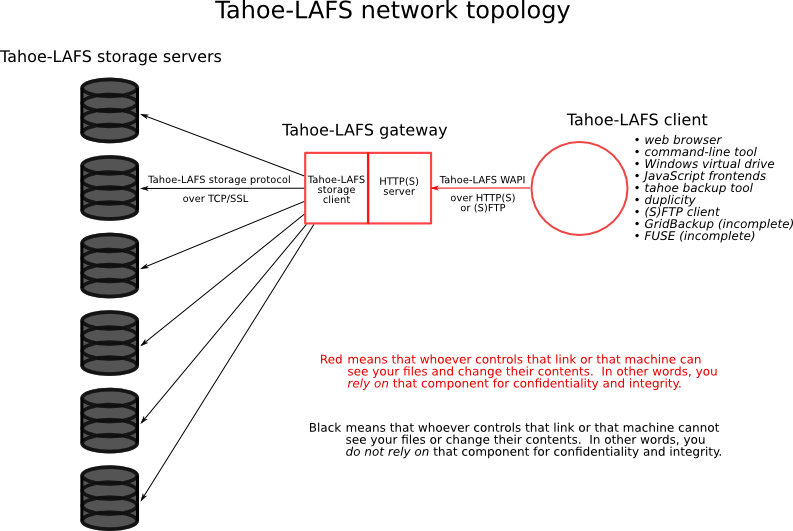
\includegraphics[width=.75\textwidth]{include/TahoeTopology.pdf}
  \caption{The Tahoe Topology}
  \label{fig:TahoeTopology}
\end{figure}

Tahoe could be thought of quite simply as collection of three layers: 

\begin{enumerate}
\item The lowest layer is effectively a Distributed Hash Table (DHT), 
like a python dictionary, but spread across multiple machines. In this 
DHT, there are a large number of "slots" which are filled with arbitrary 
data. Tahoe has both mutable slots and immutable slots. Immutable slots 
are write-once: after the slot has been closed, no more data can be written 
to it. Mutable slots can be written multiple times. Capability discipline 
is used to control access to the slots: if you hold a write-reference 
(or "write-cap"), then you can modify the slot, if you don't hold such a 
reference, then you cannot. Mutable slots have both write-caps and 
read-caps (and the write-cap can be used to produce a read-cap, so really 
it is a read+write-cap). Immutable slots have only read-caps. These read- 
and write- caps can be expressed as short strings, containing encryption 
keys, integrity hashes, and location information. In this form, they look 
a lot like web URIs: a string that provides a reference to some piece of 
data. The data for each DHT slot is distributed among some number of 
storage servers, using encryption and erasure coding to provide 
confidentiality and reliability. 

\item The middle layer is the Virtual Drive, which organizes these slots 
into directories. Each directory is just a table that maps a name to a 
read-cap or write-cap of some child file or subdirectory. Each client 
stores a specific "root directory" to use as a starting point. To visit 
e.g. /projects/tahoe/README.txt, the client will look up "projects" in 
the root directory, then look up "tahoe" in the results of that first 
query, then look up "README.txt" in the results of the second query, and 
finally present the contents of the file to the user. The table's child 
entries can point to any file or directory object, even itself, therefore 
allowing cycles. As a result, the virtual drive is shaped like an arbitrary 
directed graph rather than being a strict tree. Essentially, then, it keeps  
track of directory nodes to maintain a graph of files and directories. 

\item The top-most layer is an application or presentation service; 
something that uses the virtual drive for some purpose. Tahoe currently 
has two such interfaces. The most mature one is a RESTful HTTP interfaces, 
in which PUT, GET, and POST are used to add and retrieve files and 
directories. This interface provides HTML for the benefit of a human sitting 
at a web browser, and JSON for the benefit of programs using httplib. The 
other interface under development is a FUSE plugin, allowing all programs 
on a host computer to use the Tahoe virtual filesystem as if it were a local 
one. 

\end{enumerate}

\subsubsection{Tahoe Design Considerations}
Tahoe's primary goal is to provide safe, reliable storage of data. This comes 
at a cost: redundant shares and periodic repair. There is a tradeoff between 
cost and reliability as more redundancy requires more hard drives and more 
servers, but reduces the likelihood of data loss. The task of the designer 
is to make an educated decision between the costs and the benefits and 
choose accordingly. In addition, there are some other shortcomings of the 
system that need to be considered as part of the design/choice process. They 
are discussed in some detail below.

Although Tahoe is a distributed file system, it is not entirely 
decentralized in the strictest sense of the word. It needs a central node, 
called an Introducer, which is responsible for getting new nodes connected 
to existing nodes on the grid. Tahoe is designed to minimize its dependency 
on the Introducer, but it's still a central point of failure. If the 
Introducer fails for any reason, existing nodes will still be able to 
communicate with each other and propagate data, but the grid won't be able 
to connect new nodes. The developers hope to address this limitation in a 
future version.

Also, Tahoe provides very little control over on which nodes data is 
stored, which makes it unsuitable for tiered functionality applications. 
Furthermore, Tahoe assumes a flat local network environment and, 
therefore, is not suitable to run in a WAN. 

Tahoe is currently being used in a number of different ways. A common 
configuration that is documented at the project's wiki is described as a 
"friendnet", a group of roughly ten nodes that are connected over the 
Internet and provide shared secure storage capacity with optional 
filesharing. Another potential usage scenario is installing Tahoe on 
individual workstations on an office network and using their excess disk 
capacity as a storage pool. The Tahoe wiki describes that kind of setup 
as a "hivecache". The Tahoe source code is primarily written in Python 
with the Twisted framework. The code base is highly portable and can 
run on Windows, Mac OS X, Linux, Solaris, and several flavors of BSD and 
is now part of the Ubuntu Linux distribution. It runs entirely in user 
space and doesn't require any kernel modules or other low-level components. 
It works well on regular commodity hardware and doesn't have any 
particularly special requirements. Installation instructions are available 
at the project's web site.


\subsection{Ceph}
% Mark
Ceph is a distributed file system originally designed by the Storage 
Systems Research Center at the University of California, Santa Cruz. 
It is developed as an open source project, with code under the GNU LGPL 
license, and, since May 2010, has its client integrated in the Linux 
kernel. The objectives of Ceph are to provide a fully distributed file 
system without a single point of failure, with a POSIX-style interface. 
It claims high I/O performance and a high level of scalability. The 
file system has three main components: the client, each instance of 
which exposes a near-POSIX file system interface to a host or process; 
a cluster of object storage devices, which collectively stores all 
data and metadata; and a metadata server cluster, which manages the 
namespace (file names and directories) while also coordinating 
security, consistency and coherence.

\subsubsection{Ceph Architecture}
Ceph's architecture consists of two main components: an object storage 
layer, and a distributed file system that is constructed on top of 
this object store. The object store provides a generic, scalable 
storage platform with support for snapshots and distributed computation. 
This storage backend is used to provide a simple network block device  
with thin provisioning and snapshots, or an S3 or Swift compatible RESTful 
object storage interface. It also forms the basis for a distributed file 
system, managed by a distributed metadata server cluster, which similarly 
provides advanced features like per-directory granularity snapshots, and a 
recursive accounting feature that provides a convenient view of how much 
data is stored beneath any directory in the system. Figure
\ref{fig:CephTopology} shows the basic Ceph topology.

\begin{figure}[htbp]
  \centering
  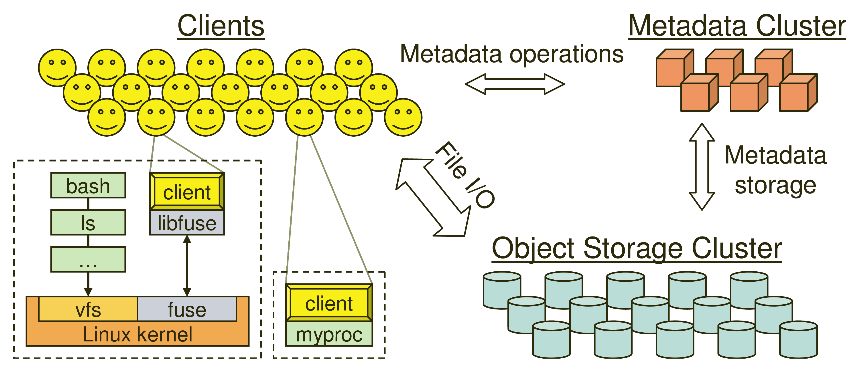
\includegraphics[width=.9\textwidth]{include/CephTopology.pdf}
  \caption{The Ceph Topology}
  \label{fig:CephTopology}
\end{figure}

The primary goals of the architecture are scalability to hundreds of 
petabytes and beyond, performance, and reliability. Scalability is 
considered in a variety of dimensions, including the overall storage 
capacity and throughput of the system, and performance in terms of 
individual clients, directories, or files. Ceph directly addresses the 
issue of scalability while simultaneously achieving high performance, 
reliability and availability through three fundamental design features: 
decoupled data and metadata, dynamic distributed metadata management, 
and reliable autonomic distributed object storage.

Ceph is based on an object storage paradigm, where file data is stored 
by object storage devices (OSDs) and metadata is stored by metadata 
servers (MDSs). Contrary to some distributed file systems relying on 
dumb’ OSDs, the Ceph OSDs have responsibilities for data migration, 
replication and failure handling and communicate between each other. 
Metadata management is completely distributed, using a cluster of MDSs 
to handle metadata request from clients. The operation is adapted 
dynamically based on the workload generated by the clients (e.g., moving 
and replicating metadata depending on how often a file is accessed).
An MDS does not keep track of which OSDs store the data for a particular 
file. Instead, Ceph uses a special function called CRUSH to determine the 
location of objects on storage nodes: it first maps an object to a 
placement group, and then calculates which OSDs belong to that placement 
group. While doing so, it takes care of the replication of file data on 
different OSDs. CRUSH automatically takes into account that the set of 
storage nodes is dynamic over time. To clients, the data within a Ceph 
configuration (potentially consisting of thousands of OSDs) is presented 
as a single logical object store called RADOS. Replication of data is 
organized by writing to the first OSD in the placement group, after which 
this OSD replicates the data to others. The client receives a notice when 
all data has reached the buffer caches on all OSDs, and receives a commit 
when the data has been safely stored on all involved OSDs. RADOS has 
mechanisms for failure detection and automatic re-replication. Furthermore, 
Ceph implements a mechanism for recovery in case of system outages or 
large configuration changes.

\subsubsection{Ceph Design Considerations}
A Ceph cluster consists of a few different pieces: the monitors (mons), 
storage nodes (osds), and metadata servers (mds). One each is the minimum 
requirement, but with one the system will have no redundancy. The storage 
nodes will store the actual data on the disk. The minimum requirement 
here is two if the system is to have any redundancy across nodes. Each 
storage node is essentially an instance of the Ceph-OSD, providing access 
to a local disk or set of disks. The simplest option is to use one Ceph-
OSD daemon per hardware node and then pool the disks. Ceph generally is 
found to work best when using BTRFS, but other file systems like ext3 and 
ext4 represent other viable choices. Btrfs provides checksumming and the 
ability to pool disks together without RAID, can internally handle data 
redundancy and facilitates Ceph journalling. 

The Ceph Metadata Server functions as a distributed, cache of file system 
metadata. It does not store data locally, rather all metadata is stored on 
disk via the storage nodes. MDS daemons can be added into the cluster as 
needed. Typically guidelines suggest starting with 1 or 2, then add more 
as necessary. The 'max mds' parameter controls how many cmds instances 
are active. Additional running instances are put in standby mode. The 
Ceph Monitor daemons administer central cluster management, configuration, 
and state. Data is stored in a directory on the local host file system. 
They must be deployed in odd-number sets. One daemon is acceptable; three 
is ideal for most use cases. More may be required for extremely large 
clusters. Other general cluster suggestions are: (1) For a few nodes,  
put Ceph-MON, Ceph-MDS, and Ceph-OSD on the same node(s). (2) For more 
nodes,  put Ceph-MDS and Ceph-MON together, and Ceph-OSD on the disk nodes. 
(3) For even more nodes, separate Ceph-MDS, Ceph-MON, and Ceph-OSD all 
onto dedicated machines.

Distributed file systems, such as  Lustre and Ceph  usually export a 
single file namespace to multiple end-users. These systems tend to be very 
complex, as they must support all file system related semantics in a 
distributed environment. To control this complexity, they are built in a 
hierarchical manner: a small number of servers store all file and directory 
metadata and the physical location of every file block, while a potentially 
large number of storage servers store the actual data. Most such systems 
cannot take full advantage of the processing and memory resources of storage 
servers, relying instead on very powerful metadata servers.  As a result, 
they do not scale well, as the small number of metadata servers often 
represents a single point of bottleneck and failure. In addition, their 
hierarchical structure often dictates a static view of the computer cluster, 
which also results in potential scaling problems. 

A major drawback is the immaturity of Ceph as a platform: by all acccounts 
in the published literature, it has not been widely used in a production 
environment, and the Ceph documentation also explicitly warns of the beta 
state of the code. Another issue is the uncertainty about the operation 
of Ceph in a WAN environment. The placement of the file data at OSDs does 
not take into account that links between storage nodes have variable 
quality (bandwidth, latency). Additionally, the operation of the mechanisms 
for automatic adaptation (adjustment of placement group to OSD mapping, 
and failure detection) may be non-optimal or worse for a WAN Ceph 
configuration.

\subsection{Lustre}
% Mark and Brendan
Lustre is a massively parallel distributed file system running on Linux 
and used at many high-performance computing (HPC) centers worldwide. 
Originally developed at CMU in 1999, it is now owned by Oracle and the 
software is available as open source under a GNU GPL license. The Lustre 
architecture defines different kinds of roles and nodes, following an object 
storage paradigm where metadata is separated from the file data. A typical 
Lustre cluster can have tens of thousands of clients, thousands of object 
storage servers (OSDs) and a failover pair of metadata servers (currently 
still a work in progress, metadata servers will in the future be able to 
form a cluster comprising of dozens of nodes). Lustre assumes that OSDs 
are reliable, i.e., use such techniques as RAID to prevent data loss.

\subsubsection{Lustre Architecture}
Lustre has a somewhat unique architecture, comprised of three major 
functional units. One is a single metadata server or MDS that contains 
a single metadata target or MDT for each Lustre filesystem. This stores 
namespace metadata, which includes filenames, directories, access 
permissions and file layout. The MDT data is stored in a single disk 
filesystem mapped locally to the serving node and is a dedicated 
filesystem that controls file access and informs the client node(s) 
which object(s) make up a file. Second are one or more object storage 
servers (OSSes) that store file data on one or more object storage 
targets or OST. An OST is a dedicated object-base filesystem exported 
for read/write operations. The capacity of a Lustre filesystem is 
determined by the sum of the total capacities of the OSTs. Finally, 
there's the client(s) that accesses and uses the file data. A diagram 
which depicts the Lustre high level architecture is presented in
figure \ref{fig:LustreTopology}.

\begin{figure}[htbp]
  \centering
  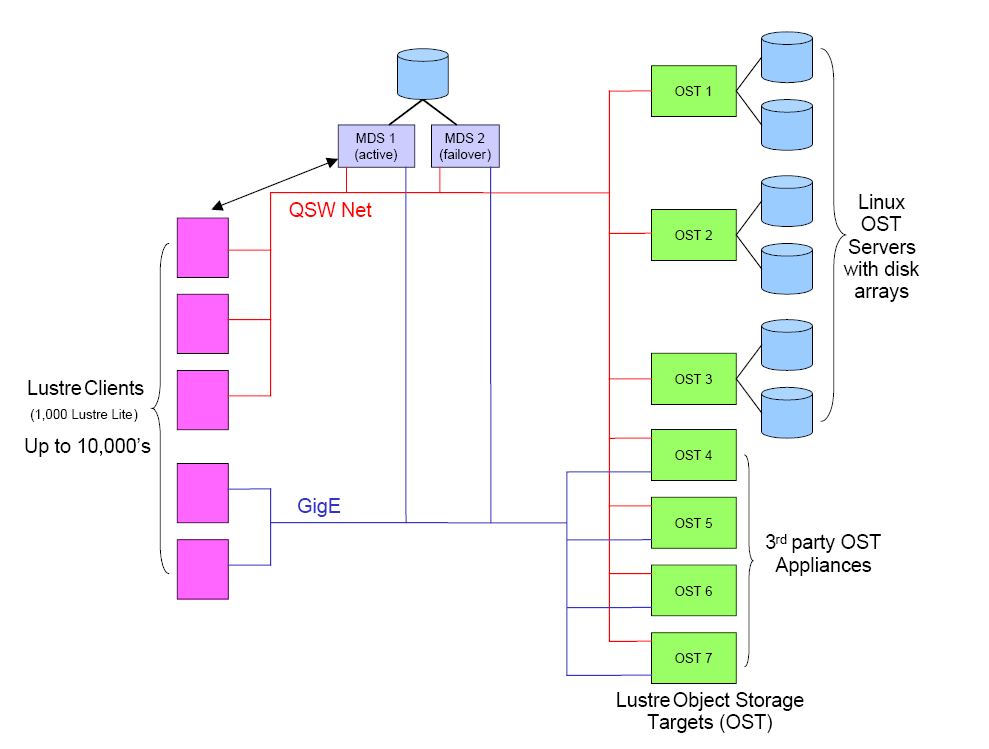
\includegraphics[width=0.75\textwidth]{include/LustreTopology.pdf}
  \caption{The Lustre Topology}
  \label{fig:LustreTopology}
\end{figure}

Lustre presents all clients with a unified namespace for all of the 
files and data in the filesystem that allow concurrent and coherent 
read and write access to the files in the filesystem. When a client 
accesses a file, it completes a filename lookup on the MDS, and 
either a new file is created or the layout of an existing file is 
returned to the client. Locking the file on the OST, the client will 
then run one or more read or write operations to the file but will 
not directly modify the objects on the OST. Instead, it will delegate 
tasks to the OSS. This approach will ensure scalability and improved 
security and reliability, as it does not allow direct access to the 
underlying storage, thus, increasing the risk of file system corruption 
from misbehaving/defective clients. Although all three components 
(MDT, OST and client) can run on the same node, they typically are 
configured on separate nodes communicating over a network.

\subsubsection{Lustre Design Considerations}
Servers can currently be added dynamically and the file system is 
POSIX compliant. Other features that Lustre provides are ADIO 
interfaces, it can disable locking, and perform direct I/O that is 
usable for databases. Lustre also has other tuneable settings. It can 
currently be installed on Linux where it can interoperate amongst all 
supported processor architectures. It is still being developed for 
other operating systems.

A file system can have one MDS and one or more OSSs, and each OSS can 
be connected to one or more OSTs. The networking layer of Luster can 
support various network connections, including Elan, Myrinet, InfiniBand, 
and TCP/IP.

File data is striped across objects on different OSTs, and users can 
configure parameters such as stripe size and stripe count to achieve 
best performance. The capacity of a Lustre file system equals the sum 
of the capacities of OSTs, and the aggregate available bandwidth equals 
the sum of the bandwidth offered by OSSs to clients. Users can extend 
storage capacity by dynamically adding more OSSs and OSTs. Data striping 
balances work load among OSSs, leading to high I/O throughput and 
excellent scalability as the number of client increases. MDSs and OSSs 
can both be configured into failover pairs with shared storage, so that 
when one node in a pair fails, the other one will take over its work load 
until it recovers. OSTs can be configured as RAID to handle disk failures 
better.

The main advantage of Lustre is that it has very high parallel 
performance, it also has good file I/O and can handle requests for 
thousands of files. Lustre does not seem to be deployed frequently 
in clusters that stretch over large distances.

The chart below provides a feature comparison of the three systems.

\begin{table}
  \begin{center}
    \begin{tabular}{
        | p{0.2\textwidth} | p{0.2\textwidth} | p{0.2\textwidth} | p{0.2\textwidth} |
      }
      \hline
      Attribute & Tahoe & Ceph & Lustre \\ \hline
      License & GNU GPL & GNU LGPL & GNU GPL \\ \hline
      Data Primitive & object (file) & object (file) &
      object (file) \\ \hline\
      Data Placement & random & placement groups, pseudo-random mapping &   
      based on round robin and free space heuristics \\ \hline
      Metadata Handling & flat & multiple metadata servers & 
      max of two  metadata servers  \\ \hline
      Storage Tiers & none & through CRUSH rules & pools of object storage
      targets \\ \hline
      Failure Handling & assuming unreliable nodes & assuming unreliable
      nodes & assuming reliable nodes \\ \hline
      Replication & server side & server side & server side \\ \hline
      WAN Deployment & numerous & no known deployment & TeraGrid (scientific
      data) \\ \hline
      Client Interfacing &  The API exposes standard GET, PUT, POST, and
      DELETE methods, supports JSON and HTML output & native client file
      system, FUSE & native client file system, FUSE, clients may export
      NFS, CIFS \\ \hline
      Node Types & client/server, an introducer, a key generator & client,
      metadata, object & client, metadata, object \\ \hline
    \end{tabular}
    \caption{System Comparison}
    \label{tbl:syscomp}
  \end{center}
\end{table}

While the features contrasted above provide a view across markedly different 
architectures and storage system applications in practice, they represent a 
robust mixture of recent, but both proven and experimental distributed file 
storage systems. As such, they illustrate many of the trade-offs we intend 
to explore in our evaluation testing.

\section{Test Setup}
Distributed storage systems may operate over a dedicated set of machines 
or may be used to acquire storage on user workstations. Potential 
implementation challenges typically result from changing conditions to 
which such systems are exposed. This can include changes in the 
available network performance, changes in the frequency at which users 
connect/disconnect their machines from the distributed storage system, 
and the frequency with which users access data. The perceived 
characteristics of distributed storage systems depend on their 
configuration parameters and on combinations of various dynamic 
conditions.

For a set of conditions, a particular configuration may be superior with 
respect to measures such as performance and resource use. Performance in 
this context is the average time required to retrieve or store data in the 
distributed storage system. In many studies comparing distributed storage 
systems, the focus is often on network resources which are consumed by the 
distributed storage system. The ratiomnale is that network resources are 
generally exhausted faster than storage or computational resources in many 
usage scenarios. For example, it is assumed that network bandwidth is a 
scarce resource in a wide-area distributed storage system. The overall 
performance and resource consumption of a distributed storage system though, 
generally depends on the performance of its individual components and, more 
specifically, on individual parts of these components.

One part of a distributed storage system whose performance and resource 
consumption depends on a specific configuration parameter is the data 
retrieval mechanism. This configuration parameter is the degree of 
concurrency with which data is retrieved. The degree of concurrency 
controls the aggressiveness with which multiple redundant replicas 
are retrieved. Two unfavorable situations can be identified. One occurs 
when the degree of concurrency is low and there is a large variation in 
the time taken to retrieve replicas. In this case one should increase the 
degree of concurrency, since, by doing so, more replicas can be retrieved 
in parallel and a result can be returned to the user more quickly. 
Similarly, when the degree of concurrency is high, there is little 
variation in retrieval time and there is a network bottleneck close to 
the requesting client. In this case it is advantageous to decrease the 
degree of concurrency, since the low variation negates the benefit from 
parallel retrieval, and the bottleneck means that decreasing parallelism 
reduces both bandwidth consumption and the elapsed time of the user.

The above demonstrates a case where a specific configuration is beneficial 
with respect to performance and resource consumption for a given set of 
circumstances but ceases to be so as conditions vary. In such situations 
a dynamic adjustment to the configuration may be more useful than a static 
configuration driven by human intervention. Due to its complexity and 
dynamic nature, this configuration adjustment of a distributed storage 
system ideally occurs automatically. In the cases of systems we are 
reviewing, this dynamic configuration adjustment capability exists in 
each respective system to varying degrees. In the subsections below we 
describe the initial test system setup as well as the initial 
configuration setup for each of the systems being reviewed. Subsequent 
parameter adjustments, made either dynamically or statically, are not 
discussed.  

\subsection{Tahoe Test Environment}
% Andy + Bryan

\begin{table}
  \begin{center}
    \begin{tabularx}{\textwidth}{|X|X|X|X|X|}
      \hline
      {\bf Name} & {\bf CPU} & {\bf Memory} & {\bf HD} & {\bf OS} \\ \hline
      xpc1 & Intel P4 3.00 GHz & 2x512GB DDR400
      & DiamondMax10 160GB SATA & Ubuntu 11.10 x64 \\ \hline
      xpc2 & Intel Celeron D 2.93 GHz & 1x1GB DDR400
      & DiamondMax10 160GB SATA & Ubuntu 11.10 x64 \\ \hline
      xpc3 & AMD Semperon 3000+ & 2x512MB DDR400
      & DiamondMax10 160GB SATA & Ubuntu 11.10 x64 \\ \hline
    \end{tabularx}
    \caption{Testbed Machines}
    \label{tbl:testbed}
  \end{center}
\end{table}

The Tahoe test environment consist of three micro-ATX PCs. Their
characteristics are available in Table \ref{tbl:testbed}. Each machine
is running the latest desktop version of Ubuntu 11.10 as of the time
of this writing (Early April, 2012).
Each machine has an identical 160GB SATA 3.0 Gb/s hard disk
partitioned in the following manner using an MBR partition table:

\begin{packed_item}
\item {\bf sdX1} - 1 GB - primary - Swap partition
\item {\bf sdX2} - 60 GB - primary - ext4 OS partition
\item {\bf sdX3} - 100 GB - Extended partition table for LBA partitions
\item {\bf sdX5} - 30 GB - logical - ext4 - Tahoe Data partition
\item {\bf sdX6} - 30 GB - logical - TBD - Unused
\item {\bf sdX7} - 30 GB - logical - ext4 - Unused
\end{packed_item}

\begin{figure}[htbp]
  \centering
  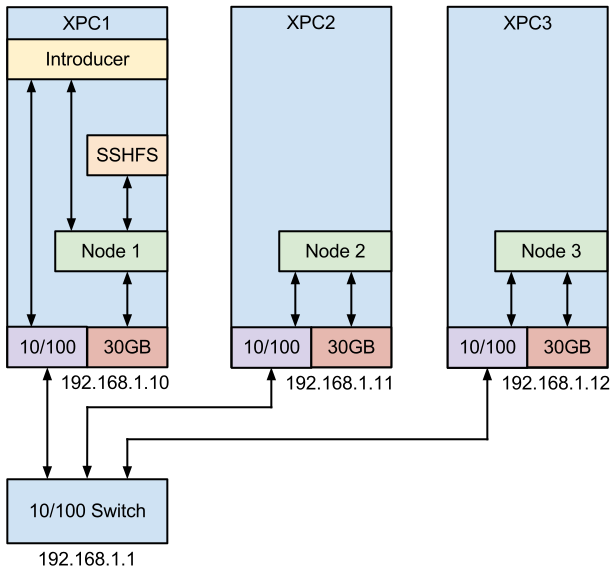
\includegraphics[width=0.6\textwidth]{include/TahoeTestbed.pdf}
  \caption{Our Tahoe Testbed Setup}
  \label{fig:TahoeTestbed}
\end{figure}

Figure \ref{fig:TahoeTestbed} shows our testbed setup.
All machines are connected to
each other via a 10/100 IPv4 Ethernet network connected to a
Cisco Linksys WRT110 Switch. The network is local and shared only by
the three test machines and the switch. The switch also acts as a
router, gateway and firewall, regulating traffic to and from the Internet.
The machines use static IP addresses:

\begin{packed_item}
\item {\bf xpc1} - 192.168.1.10
\item {\bf xpc2} - 192.168.1.11
\item {\bf xpc3} - 192.168.1.12
\item {\bf Switch} - 192.168.1.1
\end{packed_item}

When running tests, we attempted to insure that each machine was
performing no extra work other than the work required to run the
benchmark and the backing file system under test. We also attempted to
separate the behavior and performance of the various file systems
under test to avoid cross-effects between the systems. Thus, only one
file system was tested at a time, and all other file system were
isolated to their own partition and shutdown while these tests were
occurring. 

XPC1 is serves as both a Tahoe Introducer, and a Tahoe data node. XPC2
and XPC3 serve only as headless data nodes. XPC1 also serves hosts our
primary interface to the Tahoe system: the Fuse SSHFS filesystem. This
system provides a POSIX VFS compatible mount point into teh Tahoe
system, allowing us to run tests as though it were a standard Unix
filesystem.

\subsection{Ceph and Lustre Test Environment}
The Lustre/Ceph tests were conducted in a separate test environment from
Tahoe due to the need for xvery specific resources.The objective in the 
evaluation was to evaluate a few straightforward use cases in a wide area 
setup with a limited number of nodes. We realize that a limited test 
environment as used here is not capable of supporting a broad number of 
scenarios and limits the conclusions that can be drawn particularly with 
respect to performance behavior across a more industrial strength 
implementation as well as related issues like fault tolerance; such a test 
would require a very large setup and considerably more resources to execute 
than we could secure for this project. Notwithstanding that fact, the test 
environment is briefly described below. 

The experimental evaluation of our system was conducted in a cluster of 14 
identical PCs with dual core CPUs running at 1:2 GHz, 1 GB RAM, 1 HDD 
spinning at 7200 rpm and 1 Gbps Ethernet cards. All PCs were directly 
connected to a Gigabit Ethernet switch (HP ProCurve 1810g). The bandwidth 
measure-ment benchmarks conducted in the evaluation environment using netperf 
indicate a maximum data rate between two PCs (full-duplex) of about 800 Mbps. 
For the Ceph system tests, we used the Ubuntu 10:04 distribution. For Lustre 
tests we used Ubuntu 8:10 with the patched kernel provided at the Lustre 
website.

\subsection{Tahoe - Installation and Configuration}
% Andy + Bryan

Using our environment setup of three computers all running Ubuntu
11.10 with a partition mounted for use by the Tahoe Filesystem at
/Tahoe we could begin to setup the Tahoe Least Authority File System.

\begin{enumerate}
\item The first step for deploying Tahoe was to acquire the latest
  version of the Tahoe LAFS from their website for each of the
  computers. \cite{tahoe-lafs.org} At the time this was version
  1.9.1. Once we had downloaded the \texttt{allmydata-tahoe-1.9.1.zip} file
  from the Tahoe LAFS website, we could move onto the next step.
\item The second step was to insure we had a compatible version of
  python installed on all the computers. \cite{python.org} For the
  installation of the Tahoe LAFS version 2.4.4 or greater is
  required. And Python v3 or greater would not work either. Python
  2.7.2 was already installed on Ubuntu 11.10 so we could move onto
  the next step.
\item We now extracted the Tahoe LAFS source files from the
  \texttt{allmydata-tahoe-1.9.1.zip} file we acquired from their website. This
  resulted in a folder in our home directory, which is where we
  downloaded the file on each computer, called \texttt{allmydata-tahoe-1.9.1}.
\item Now that we had the Tahoe LAFS source extracted we could build
  the tahoe executable using the following command inside the
  allmydata-tahoe-1.9.1 folder to build the source via the python
  setup file.
\begin{verbatim}
python setup.py build
\end{verbatim}
\item After the build had finished we got a subdirectory called bin
  inside the source directory that contains the tahoe executable that
  is used to initialize and start, run, and stop the tahoe introducer
  and clients. We now repeated this build process on the remaining
  computers.
\item Now that we have the tahoe executable created on all the
  computers we needed to decide which computer was best suited to be
  the introducer as it will have a slightly heavier load as it will
  act as the node the clients connect to and due to our limited number
  of computers we will also have a client node running on it as
  well. We chose to use computer XPC1 for this due to the
  observational behavior of it was significantly more responsive than
  the other two computers, eventually a performance benchmark will be
  run on each of the computers to determine that this was the correct
  choice. As we wanted to get something up and running we went ahead
  on this assumption to see if we could get the Tahoe LAFS working on
  these computers.
\item The next step was to create subdirectories on XPC1 for the
  introducer and client to use as each will have their own
  configuration files. To this end an introducer and client directory
  were created in the \texttt{/tahoe} directory. The creation of a client
  directory could be done on the other two computers could be done as
  well to make the commands used to get the Tahoe clients running
  consistent across all three computers; however, at this time this
  was not done.
\item The next step was to get our introducer node created as we need
  it running before we can properly setup the client nodes. To create
  the introducer node we used the following command from the
  \texttt{~/allmydata-tahoe-1.9.1/bin} directory where the tahoe executable
  lives: 
\begin{verbatim}
tahoe create-introducer --node-directory=/tahoe/introducer
\end{verbatim}
This creates the introducer configuration files inside the
/tahoe/introducer folder and will allow us to edit the \texttt{tahoe.cfg} file
with the configuration tweaks we need to make for our small number of
available nodes.
\item The next step is to edit the \texttt{/tahoe/introducer/tahoe.cfg} file to
  include the following changes:
\begin{verbatim}
...
nickname = xpc1
web.port = tcp:3457:interface=127.0.0.1
shares.happy = 2
...
\end{verbatim}

These changes give the introducer a nickname that we can recognize and
also provides us with a web interface port that is different from the
default port for tahoe interfaces of \texttt{3456} so that eventually we will
be able to see both the introducer and client's web interface for XPC1
with out them conflicting on the same port.

\item After we had made the necessitated changes to the introducer's
  \texttt{tahoe.cfg} file we saved it and could start the introducer
  running. This is necessary for the clients to be able to connect to
  the introducer, but also because it needs to be started at least
  once before the \texttt{introducer.furl} file is created. This is needed in
  the client configuration as this is how the clients find the
  introducer and function as a group. To start the introducer running
  we use the following command assuming we have added the tahoe
  executable to the path:
\begin{verbatim}
tahoe start --node-directory=/tahoe/introducer/
\end{verbatim}

\item Now that we have the introducer running on XPC1 we are ready to
  create the client nodes. Instead of creating clients, we opted to
  just create nodes that share their storage vs only replicate their
  files across the available nodes as we only have three working
  computers. To create a node we used the following command on XPC2 \&
  XPC3:
\begin{verbatim}
tahoe create-node --node-directory=/tahoe/
\end{verbatim}
And we used this command on XPC1:
\begin{verbatim}
tahoe create-node --node-directory=/tahoe/client/
\end{verbatim}
This created all the configuration files for the client nodes in their
respective directories.

\item Now that we have the client directories created we want to open
  up the \texttt{introducer.furl} file and copy out the
  enclosed furl in the file so that we can put it in the client
  \texttt{tahoe.cfg} files. For our introducer we have the following contents
  for the \texttt{introducer.furl} file:
\begin{verbatim}
pb://6n56ctw77txdhrc2455jnwe3zzouho6n@192.168.1.10:57307,127.0.0.1:57307/introducer
\end{verbatim}

\item We now open up the clients \texttt{tahoe.cfg} file and edit it to reflect
  the following changes, with what is in the [ ] indicating a value
  that varied between computers or is too long to fit below:
\begin{verbatim}
...
nickname = [name of computer]
introducer.furl = [contents of introducer.furl]
shares.happy = 2
...
\end{verbatim}
With these changes our clients are ready to be started and have been
configured to be able to work on our extremely small grid.

\item The final step is to start the client nodes. We are going to use
  the command to run the tahoe client nodes in the background;
  however, it is worth mentioning that there is a command that would
  run it in the foreground in a UNIX environment instead that was used
  during our initial test run to see if the Tahoe LAFS was working. To
  start the clients on XPC2 \& XPC3 the following command was used:
\begin{verbatim}  
tahoe start /tahoe/
\end{verbatim}
And on XPC1 the following command was used:
\begin{verbatim}
tahoe start /tahoe/client/
\end{verbatim}
This started the client nodes running in the background and our Tahoe
LAFS grid is now installed, configured, and running.
\end{enumerate}

Now that we had the Tahoe LAFS running we verified that it was working
by navigating to \texttt{127.0.0.1:3457} on XPC1 to verify that the introducer
was working and check on its status. It showed us that it was running
and that the three client nodes were connected. We then went to the
web interface for the client node on XPC1 located at \texttt{127.0.0.1:3456}
that provided us with an interface to upload \& download files, create
directories, and showed us the status of the available storage
nodes. We then uploaded an image file to verify that we could upload a
file and then download it again. We were able to successfully retrieve
the image file back out of the Tahoe LAFS. This was done to insure
that we had in fact installed, configured, and gotten the Tahoe LAFS
working.

To expedite starting and stopping the Tahoe cluster during testing, we
wrote series of scripts that remotely start and stop all Tahoe nodes in the
correct order. These scripts also take care of starting the Introducer
and insuring that the SSHFS mount is up and running. Copies of the
scripts are included in Appendix \ref{sec:TahoeScripts} in Listings
\ref{lst:sshpw} through \ref{lst:stop-tahoe-xpc3}.

\subsection{Ceph - Installation and Configuration}
% Mark

Most Ceph installation guides recommend that the storage daemons in Ceph 
use btrfs for storing data and taking advantage of btrfs' internal 
transactions to keep the local data set in a consistent state. The claim 
is that this makes the storage cluster simple to deploy. In addition it 
is intended to provide scalability not currently available from block-
based Linux cluster file systems. Ceph provides some new features for 
Linux-based users. Directory snapshots provide users with the means to 
create read-only snapshots of directories and their nested contents using 
the command 'mkdir .snap/my\_snapshot'.  Deletion is also a simple task 
using the command 'rmdir .snap/old\_snapshot'.  Ceph also provides 
statistics on the number of nested files, directories, and file sizes 
for each directory. This makes it fairly easy to manage usage in the 
system.

Ceph uses a single configuration file to define cluster membership, 
hostnames, paths to devices, and runtime options. The configuration 
file is designed so that everything can be placed in a single file and 
shared unmodified on all hosts in the cluster. Hence, no per-node 
configuration file changes should be necessary. The default location 
for the configuration file is /etc/ceph/ceph.conf. A single master 
ceph.conf file that contains configuration information for the entire 
cluster can be maintained, and then configured by  a 'fetch\_config' 
script on each node that will pull down the configuration when it is 
needed. For command line user tools (e.g., 'ceph'), you can define an 
/etc/ceph/ceph.conf that contains at a minimum the monitor ip addresses, 
as that is usually all you need. A different configuration file can be 
used on each host, defining parameters only for the daemons running on 
that host, but this is more difficult to maintain. The one point is that 
the configuration file on every host should include the monitor daemon 
sections and 'mon addr' option, so that the daemon knows how to join the 
cluster. Other monitor options can be omitted, except, of course, on the 
hosts running the monitors themselves.

Some other general configuration tips include: (1) ensuring that the log 
partition is on a fast disk as Ceph produces a large quantity of logs, 
and, (2) enable noatime everywhere, particularly on the OSD store.
In creating a new file system, the --mkbtrfs option will create a new 
btrfs file system for each OSD and mount it for you. It requires that 
the 'btrfs devs' and 'btrfs are specified. Since no safety checks are 
made, one needs to be careful with the 'btrfs devs' option. To use ext4 
instead of btrfs, comment out "btrfs devs" in ceph.conf, point "osd data" 
to an already mounted ext4 partition and use mkcephfs without --mkbtrfs. 
The ext4 partition must be mounted with -o user\_xattr or else mkcephfs 
will fail. Also using noatime, nodiratime boosts performance at no cost. 
When using ext4, you should disable the ext4 journal, because Ceph writes 
its own journals. This step can enhance performance.  Creating a new file 
system on an ext4 partition that already contains data, will invoke rm -rf 
to delete the data. If there is a lot of it, it might seem as if mkcephfs 
is hanging when it actually is not. The -k admin.keyring option lets you 
specify where mkcephfs puts your master admin key file. This is needed to 
administer the cluster when authentication is enabled. Various keys are 
generated even if authentication is disabled, so that it can be enabled 
later. 

Ssh keys need to be setup so that the machine running mkcephfs (the master) 
can ssh in to other nodes as root. The usual way to do this, assuming no 
authorized\_keys are set up, is to generated the public/private key pair and 
then ssh it to other slaves as the root. Once the file system is created and 
the Ceph daemon is running, it must be mounted. This done using the kernel 
driver or with fuse. The monitor is always mounted. From there, getting a 
simple test cluster to start up out of your source directory is relatively 
straightforward.

Like most distributed file systems, Ceph doesn't deal well with OSDs that 
run out of space. To prevent even-more disastrous scenarios from occurring, 
once an OSD reaches pre-defined thresholds of disk usage the monitor will 
set a full flag on the OSDMap. Once that flag is set’ the OSDs will reject  
all client writes and all clients will pause writes. There are a few things 
that can be done to improve things in this situation: (1) Rebalance the data 
by reweighting the OSDs, and (2) Increase the thresholds for the full flag.
Since the Ceph MDSes are essentially a single point of failure, there is a 
need to ensure that they recover quickly. To do this, Ceph supports the 
standby-replay mode. Herein, an MDS in standby-replay will continuously 
replay the journal of an active MDS. This does the following two things: 
(1) ensures that the journal is tested. If there are problems with it, the 
MDS will error out and a bug can be filed. (2) If the active MDS fails, the 
standby-replay takes over. Since it has already cached the appropriate 
metadata, it doesn't need to replay the entire journal.

Ceph is a complex project, with many independent components. Different parts 
of the system are tested differently. At the lowest level, functional and 
minimal units of code are tested with unit tests. Unit tests are isolated 
from the real world in the sense that they do not use networking, special 
kernel features or such. This helps keep them fast, safe and easy to run.  
For simple command-line tools doing basic file manipulation, unit tests are 
difficult to write and integration tests represent test overkill. This is 
where cli tests come handy. The idea is to write the command to run, the 
expected output, and the expected exit code in a file. Organize tests based 
on the command line tool they are (primarily) testing. The cli tests can be 
run "./src/test/run-cli-tests", or just "make check". Also check out the 
interactive mode of cram, that can helps you update tests when there are 
trivial changes -- do take care to read carefully still, and not just 
blindly accept the new output.  Additionally the tester should note that 
interactive mode can lose carefully crafted regexps. In more complex cases, 
testing may require regular expressions. This is done by adding "(re)" at 
the end of the line.

\subsection{Lustre - Installation and Configuration}
% Mark + Brendan

In building Lustre from source, one needs to ensure that they are using 
Linux kernel 2.6.16 or greater. In all deployments of Lustre, the server 
that runs on an MDS, MGS or OSS needs to utilize a patched kernel. 
Running a patched kernel on a Lustre client is optional and required only 
if the client will be used for multiple purposes, such as running as both 
a client and an OST. The /boot/grub/grub.conf file needs to be reviewed 
to validate that the newly installed kernel has been set as the default 
kernel. Once all packages have been installed, a reboot is required to 
load the new kernel image. Once the system has been rebooted, an invocation 
of the uname command will reveal the currently booted kernel image. With 
respect to the client side, the packages for the lustre client and lustre 
client modules need to be installed on all desired client machines. Client 
machines need to be within the same network as the host machine serving the 
Lustre filesystem. After the packages are installed, a reboot must be 
performed on all affected client machines.

To configure the Lustre filesystem, one needs to configure Lustre Networking, 
or LNET, which provides the communication infrastructure required by the 
Lustre filesystem. LNET supports many commonly used network types, which 
include IP  networks. It allows simultaneous availability across different 
network types with routing between them. Note the role of the Management 
Server or MGS. The MGS stores configuration information for all Lustre 
filesystems in a clustered setup. An OST contacts the MGS to provide 
information, while the client(s) contact the MGS to retrieve information. 
The MGS requires its own disk for storage, but a provision exists to allow 
the MGS to share a disk with a single MDT. If nothing is provided then the 
default fsname is lustre. If one or more of these filesystems are created, 
it is necessary to use unique names for each labeled volume. These names 
become important for when one accesses the target on the client system.
The OST is created by executing a set command. When the target needs to 
provide information to the MGS or when the client accesses the target for 
information lookup, one needs to be aware of where the MGS is, which is 
defined for this target as the server's IP address followed by the network 
interface for communication. At this point one can mount newly formatted 
devices local to the host machine using a generic mount command. When one 
mounts the volume over the network on the client node, one must specify 
this name. This is done by following the network method by which the 
remote volume is mounted. Once mounted, the file system can be accessed 
by the client node. What that implies is that one cannot read or write from 
or to files located on the mounted OST. 

What is described above is a simple description of installing and 
configuring the Lustre distributed filesystem; a more full accounting 
is beyond the scope of this paper. Of course, richer implementations are 
possible. For example, Lustre can be configured for high availability to 
ensure that in the situation of failure, the system's services continue 
without interruption. That is, the accessibility between the client(s), 
server(s) and external target storage is always made available through 
a process called failover. Such high availability is provided through 
an implementation of disk drive redundancy in some sort of RAID 
configuration for the event of drive failures. 

In short, Lustre isn't a particularly difficult technology to work with 
since there is an established community with excellent administrator 
and developer resources ranging from articles, mailing lists and more 
to aid in installation and maintenance issues that may arise. Also, 
commercial support for Lustre is provided by a large number of vendors 
who sell bundled computing and Lustre storage systems. Many of these 
vendors also contribute to the open source community's Lustre Project. 

\section{Evaluation}
\subsection{Introduction}
Storage technology is developing rapidly, but the corresponding 
measurement technology is seriously lagging behind. Interestingly enough, 
this impedes the development of storage industry. The absence of uniform 
evaluation tools and evaluation methods, coupled with storage vendors who 
do not make available all relevant metrics for an application and its
environment creates a situation where a user can not accurately select 
storage products to address a particular needs. Hence, firms and users 
often spend significant amounts of money but often get a product which 
exhibits low system performance, directly impacting firm profitability. 
Since slow storage performance implies slow response times and longer 
running queries, slow storage negatively impacts customers while 
squandering the investments made in server infrastructure. Conversely, 
inappropriate use of fast storage translates into wasted dollars spent 
on performance.

The issue is that performance testing for a distributed storage system 
is an important and valuable undertaking. Also, though, storage system 
performance testing is a very complex task, because it is affected by 
a myriad of factors: such as block size, file size, queue depth, number 
of threads, read / write ratio, random / sequential ratio, in addition, 
the disk’s speed, cache size, caching mechanism, cache algorithm, bus 
bandwidth, the number of disks, RAID level, and storage protocol, all 
of which will affect the performance of storage system. Therefore 
relying on one benchmark to measure the performance of distributed 
storage system has limitations. Rather, to fully test the performance 
of a distributed storage system, we fiollow the lead of others and 
choose a variety of benchmarks. The hope is that this approach will 
make the test results more realistic, reliable and credible.

The intent of the testing phase is to understand the tradeoffs that 
the various systems under review make in architectural design and 
observe how those design choices translate into performance and 
resource usage in actual operation.

\subsection{Test Implementation}
The Linux test platform will test the file system IO performance, 
including the aggregate bandwidth, the amount of concurrent access, 
and the throughput of metadata. The user can set the file size, 
transfer block size, file system API, and then select the test nodes 
to start the testing task, which can measure the file system IO 
performance. The test platform is also able to test the disk array 
IO performance, including the IOPS and the DTR of disk array. The user 
can set the queue depth, number of threads, transfer block size, 
random/sequential ratio, read/write ratio, and then select the tested 
disk and test nodes to start the testing task, which can measure the 
IO performance of disk arrays.

The following is the set of test steps for the distributed file system.
The first is to select the test benchmarks. Recall that different 
performance indicators, such as the aggregate bandwidth, the amount of 
concurrent access and the metadata throughput have different benchmarks. 
The second is to specify parameters for configuration. Each benchmark 
has its own testing parameters. The third step is to select the tested 
object (the target distributed file system) and the test nodes. The 
fourth step is to start the test and display the corresponding test 
results. The fifth step is to generate the reporter and display the 
test result in graphics. Finally, all the test results and test 
parameter configurations need to be stored in a database, so that the
user can easily query and compare the test results.

In addition, in order to manage and monitor the testing tasks in a 
comprehensive manner, the test platform needs to be able to manage 
all the test nodes, as well as monitor the performance of test nodes. 
That is, users need to be able to dynamically add or remove test 
nodes to meet the scale of testing task. 

\subsection{Tahoe Tests}
% Andy

To test the throughput and latency of the Tahoe system, we used a
combination of the Unix \texttt{dd} utility. Timing instrumentation
was provided via GNU \texttt{time} and \texttt{date}, and the built-in Tahoe
instrumentation. We ran a series of tests using various file sizes
from 1 MiB to 3 GiB. We also tested the system using both random data
(as provided via \texttt{/dev/urandom}) and zeros data (as provided
via \texttt{/dev/zero}). We tested for read and write throughput, and
write latency.

To find the base read and write throughput, we used the \texttt{dd}
utility with a 1024 byte block size. Calls to \texttt{date} were used
to clock the start and end time of the test. For read tests, this looked like:
\begin{verbatim}
date;
dd if=<Tahoe File> of=\dev\null bs=1024;
date;
\end{verbatim}
For write tests, this looked like:
\begin{verbatim}
date;
dd if=\dev\urandom of=<Tahoe File> bs=1024 count=<size>;
date;
\end{verbatim}

These tests provided raw read and write speeds for specific file sizes
and data types. On writing to Tahoe, however, files are not available
immediately after the \texttt{dd} write completes. Instead, there is an
additional latency between the completion of the \texttt{dd} write
and the availability of the written data. This delay is due to the fact
that Tahoe must propagate the written files to all necessary nodes
before they are available for reading. This operation is not pipelined,
instead it begins as soon as the \texttt{dd} write completes. Thus, we
had to use the Tahoe file timestamps to record when the file became
available on the Tahoe system, and thus how much time had elapsed
since the completion of the \texttt{dd} write. This additional time
metric was used to compute the write latency, or overhead throughput, of the
Tahoe system.

In addition to the base read throughput, the base write throughput, and the Tahoe write
overhead throughput, we also calculated the end-to-end write
throughput. This was calculated by simply dividing the size of the
test file by the difference
between when the \texttt{dd} write started and when the data became
available via Tahoe. There is no relevant equivalent read metric, as data need
not propagate across the Tahoe cluster when being read. Thus the
end-to-end read throughput is always equal to the base \texttt{dd} read
throughput.

\subsection{Ceph and Lustre Tests}
In this subsection we evaluate the I/O performance of the Ceph and 
Lustre distributed file systems. In order to keep the measurements 
as comparable as possible we used simple I/O workloads (i.e. sequential 
and random access patterns). The comparison gives us general indications 
regarding the potential advantages of each system and some of their 
architectural constraints. The measurements were captured using the IOzone 
tool. The Iozone benchmark tool generates and measures a variety of file 
operations. For instance read, write, re-read, re-write operations can be 
used to provide a broad analysis of filesystem performance. Iozone can work 
in a single client mode and cluster mode where it is provided with a list of 
nodes on which it will run. Iozone tests were run with a 1MB block size.  
In order to make the results as comparable as possible, each system was 
configured as follows. Our system used 13 storage nodes and a single VDD. 
All nodes were aware of each other and no overlay routing was allowed. The 
deployment did not support chunk replication. For all distributed filesystems, 
we used 13 storage devices, 1 metadata server running on a host that also acts 
as a storage device, and a single client. In all cases, clients ran in a 
dedicated PC and no other network traffic was produced simultaneously. The 
chunk size supported by our system was configured to be 256 KB, the same 
as the file stripe size for Lustre. We also measured Lustre performance 
with no file striping at all. Ceph’s current implementation does not support 
stripe configuration, therefore we used the default of 1 MB. For that reason, 
as observed below, in some cases Ceph outperforms all other systems. Ceph’s 
present deployment was configured to store a single copy of each file stripe. 
Finally, it should be noted that experiments were conducted multiple times and 
the average values are what is presented in all figures and tables.

In order to produce these measurements, we configured the tool to first 
sequentially write an entire file to the file system exported by the storage 
system and then sequentially read the entire file back. Then, the tool writes 
random parts of the file (128 KB each) in the storage system and, finally, 
reads random parts of the same size. The request size that it passes to the 
filesystem for the sequential part of the experiment was also 128 KB; this 
size did not dramatically affect the results due to the asynchronous nature 
of the I/O. 

For direct I/O results (Figure 2), our measurements were produced using 
the same process as noted above, though the file size was maintained at 
a constant file size constant (200 MB) and measured performance for several 
I/O request sizes was performed as noted in the X-axis. While certain file 
systems may not overtly support direct I/O, since they bypass the caching 
mechanism provided by the operating system, effectively they can be viewed 
to emulate a direct I/O operation.

We also evaluated the comparative scalability of the systems. This is 
done by measuring total system throughput when multiple clients access 
the storage system simultaneously as well as the I/O throughput of a 
single client when accessing a much larger deployment of the core storage 
layer. In order to measure total system throughput we used a tool (xdd) 
which supports distributed I/O benchmarking when multiple synchronized 
clients access the storage system simultaneously. We configured the tool 
so that in each step of the experiment a number of clients which are 
increasing stepwise by two, sequentially writes and, then, reads a file 
for 30 seconds. All clients are synchronized to a timeserver in the 
cluster. For each step we calculated the sum of the I/O throughput rates 
for each client. Measurements shown represent the average values of 
multiple runs per experiment. The deployment details for each system as 
noted above in the previous subsection, except here all  hosts are used 
as storage devices. The maximum number of clients is 14, in the rare case 
where all physical hosts run a storage server as well as a client.

Finally, we tested the performance of the systems when replication is 
supported as well as during node failures and joins. Starting with 
replication, out of the distributed file systems discussed in this study, 
only Tahoe and Ceph support replication. With asynchronous sequential 
writes Ceph saturates the uplink of the client. Since the Ceph stripe size 
is two to four times larger than the chunk size supported by other 
comparable PVFS systems with replication capabilities and by Tahoe, we 
would expect that performance would be similar if two such comparable 
systems grouped date in pieces of the same size. Apart from the 
replication level, the system deployments are identical to the ones 
presented in the beginning of this section.

\section{Results}
% All

Here we discuss the relevant results from each of our three tests
systems. Full test results are available in Appendices
\ref{sec:TahoeData} through \ref{sec:LustreData}.

\subsection{Tahoe Results}
% Andy

The full set of Tahoe read and write results are available in Appendix
\ref{sec:TahoeData}. We present a illustrative subset of the results
here.

Table \ref{tbl:TahoeWriteRandom} shows write throughput speeds for files
composed of random data. The average end-to-end write throughput using
random data is 0.52 MiB/s.

\begin{table}
  \begin{center}
    \begin{tabularx}{\textwidth}{|X|X|X|X|X|}
      \hline
      {\bf Data} & {\bf Size} & {\bf Base} & {\bf Overhead} & {\bf End-to-End} \\ \hline
      random & 1 MiB & 1.02 MiB/s & 1.00 MiB/s & 0.51 MiB/s \\ \hline
      random & 10 MiB & 0.99 MiB/s & 1.11 MiB/s & 0.53 MiB/s \\ \hline
      random & 100 MiB & 0.98 MiB/s & 1.39 MiB/s & 0.57 MiB/s \\ \hline
      random & 1 GiB & 1.05 MiB/s & 1.48 MiB/s & 0.61 MiB/s \\ \hline
      random & 2 GiB & 1.03 MiB/s & 1.49 MiB/s & 0.61 MiB/s \\ \hline
      random & 3 GiB & 1.03 MiB/s & 0.41 MiB/s & 0.29 MiB/s \\ \hline
    \end{tabularx}
    \caption{'random' Write Throughput by File Size}
    \label{tbl:TahoeWriteRandom}
  \end{center}
\end{table}

Table \ref{tbl:TahoeWriteZeros} shows write throughput speeds for files
composed of zeros data. The average end-to-end write throughput using
zeros data is 0.69 MiB/s.

\begin{table}
  \begin{center}
    \begin{tabularx}{\textwidth}{|X|X|X|X|X|}
      \hline
      {\bf Data} & {\bf Size} & {\bf Base} & {\bf Overhead} & {\bf End-to-End} \\ \hline
      zeros & 1 MiB & 1.11 MiB/s & 1.00 MiB/s & 0.50 MiB/s \\ \hline
      zeros & 10 MiB & 1.20 MiB/s & 1.43 MiB/s & 0.63 MiB/s \\ \hline
      zeros & 100 MiB & 1.15 MiB/s & 1.35 MiB/s & 0.62 MiB/s \\ \hline
      zeros & 1 GiB & 1.17 MiB/s & 7.64 MiB/s & 1.01 MiB/s \\ \hline
      zeros & 2 GiB & 1.15 MiB/s & 7.56 MiB/s & 0.99 MiB/s \\ \hline
      zeros & 3 GiB & 1.15 MiB/s & 0.65 MiB/s & 0.41 MiB/s \\ \hline
    \end{tabularx}
    \caption{'zeros' Write Throughput by File Size}
    \label{tbl:TahoeWriteZeros}
  \end{center}
\end{table}

As we can see from the write data, it appears that Tahoe's compression
capabilities are kicking on for the larger 'zeros' files. Random files
are not generally compressible, so no such effect is seen there.
Files exceeding 2 GiB
also seem to suffer a significant performance hit. This may be due to
limits imposed by the amount of RAM available on our test
machines. The large files may be forcing the SSHFS system to use a lot of
swap-space since each machine was only equipped with 1GB of RAM, leading
to a performance crash above a certain file size.

Table \ref{tbl:TahoeReadRandom} shows read throughput speeds for files
composed of random data. The average read throughput using
random data is 1.32 MiB/s.

\begin{table}
  \begin{center}
    \begin{tabularx}{\textwidth}{|X|X|X|}
      \hline
      {\bf Data} & {\bf Size} & {\bf Base} \\ \hline
      random & 1 MiB & 1.54 MiB/s \\ \hline
      random & 10 MiB & 1.32 MiB/s \\ \hline
      random & 100 MiB & 1.11 MiB/s \\ \hline
    \end{tabularx}
    \caption{Random Read Throughput by File Size}
    \label{tbl:TahoeReadRandom}
  \end{center}
\end{table}

Table \ref{tbl:TahoeReadZeros} shows read throughput speeds for files
composed of zeros data. The average read throughput using
zeros data is 1.42 MiB/s.

\begin{table}
  \begin{center}
    \begin{tabularx}{\textwidth}{|X|X|X|}
      \hline
      {\bf Data} & {\bf Size} & {\bf Base} \\ \hline
      zeros & 1 MiB & 1.61 MiB/s \\ \hline
      zeros & 10 MiB & 1.53 MiB/s \\ \hline
      zeros & 100 MiB & 1.13 MiB/s \\ \hline
    \end{tabularx}
    \caption{'zeros' Read Throughput by File Size}
    \label{tbl:TahoeReadZeros}
  \end{center}
\end{table}

Tahoe read throughput tends to be about twice that of write
throughput. This is likely due to a combination of the fact that Tahoe
must propagate write changes across the network, as well as the fact
that the SSHFS interface must cache the file before uploading it. No
read data was collected for files larger than 100 MiB. The system
became unstable when we attempted to read files of this size. Again,
this may be a limitation of the system RAM size and the SSHFS interface.

\subsection{Ceph and Lustre Results}
Figure 1 below presents performance with various asynchronous I/O 
workloads. Lustre256 and Lustre0 represent Lustre with and without 
striping, respectively. The X-axis represents the size of the file 
used in each experiment, ranging from 400 MB to 2 GB, while the Y-axis 
depicts the I/O throughput in MB/sec. Note that in asynchronous I/O 
ode all systems take advantage of the caching provided by the operating 
system.

% see Figure 1

For all systems and workload types, we can see that as the size 
of the file grows, measurements tend to reach a stable throughput value. This 
is due to the caching effect fading out as the size of the data involved in 
the experiment grows. We do not present measurements for file sizes less than 
400 MB for write I/O and 600 MB for read I/O since for these sizes the 
throughput rates are extremely large due to the fact that I/O is done almost 
entirely in RAM. For all workload types we notice that other systems tend to 
perform better than Tahoe, especially when large files that exceed RAM size 
are involved in the I/O. It is worth noticing that Lustre write performance 
without striping is bounded by the maximum I/O capacity of a single hard disk. 
Ceph performs best overall since, as mentioned above, the supported file stripe 
is much larger compared to all other systems.

In Figure 2 below we present the performance of each system considered when 
IOzone uses direct I/O. Direct I/O is preferred by applications such as 
database systems that require control over the way data is written to the 
back-end storage. For direct I/O, the size of the file does not affect 
performance, since no caching is provided by the operating system. The 
critical factor for the performance in this case is the request size that 
the tool passes to the file system for reading or writing.

% see Figure 2

As observed in Figure 2, Lustre0 performs equally well as PVFS and much 
better than Ceph and Lustre when dealing with sequential write workloads. 
The maximum throughput achieved for very large request sizes is bounded 
by the maximum network throughput (about 95 MB/s). The performance of 
Lustre and Ceph is poor (about 18 MB/s); performing file operations 
directly for each filesystem request seems to be costly for these systems. 
Lustre0’s performance for the sequential read workload is comparable to 
Ceph and much better than Lustre256. It is also noticeable that PVFS 
performance collapses for request sizes larger than the supported 
file striping size. This is more likely due to TCP incast which is a 
well-documented phenomenon in high performance data centers. Lastly, 
note that even though in some cases PVFS performs better than our 
systems, it does not actually support direct I/O and, therefore, a 
direct comparison between these two systems is not really possible.

Figure 3 displays total system throughput when multiple clients 
simultaneously write a file using asynchronous I/O.

% see Figure 3

In the above comparison most systems behave very well, sustaining 
a write throughput of around 300 MB/s, while Ceph barely reaches 
the value of 180 MB/s. The most scalable deployment is that of 
Lustre when no file striping is supported, since for each client 
an idle storage device is assigned for file storage and, therefore, 
system performance increases linearly. The above results show that 
Lustre filesystem scales almost linearly with the number of clients 
up to the point of saturation of the back-end storage performance. 
Adding more clients doesn't cause much performance degradation and 
overall performance remains at a fairly good level. We do not show 
read performance, since local caching makes the results incomparable 
among the respective systems.

We also performed analysis of the total throughput of each system 
when performing direct sequential writes and reads for request sizes 
ranging from 4 to 512 KB. We observe that in all cases the total 
throughput scales well, reaching the value of 220 MB/s for writes 
and 330 MB/s for reads when the request size is 512 KB. The diagrams 
are not presented as they become fairly unreadable for larger 
request sizes. 

In all these measurements a single storage node runs in each physical 
host and, therefore, the maximum number of such nodes cannot exceed 
14.  In our test environment each storage node is aware of all other 
nodes and no routing is required. However, in larger deployments the 
core storage layer may consist of hundreds or even thousands of nodes. 
In systems which are fully decentralized, each node does not have to 
be aware of all others. But, there is a cost for this decentralization. 
That is, there is the need to route the lookups sent by virtual disk 
drivers. A detailed evaluation of that cost is beyond the scope of our 
work.

However, using the IOzone tool and the presented workloads we can 
simulate performance on a larger system. One can conclude that the 
performance of a single client does not change significantly when 
accessing a system over ten times larger. We do not provide the results 
for asynchronous Input/Output since they support the same conclusion 
noted above. It is not clear whether the slight performance decrease 
is due to the overlay routing in the larger system or to the extra 
overhead, in terms of CPU and memory, required to run additional 
virtual machines per each physical host. It is important to point out 
that this is the rare case: the system is over ten times larger but 
only a single client accesses it. Increasing system size translates 
to more storage space and processing resources and, possibly, more 
aggregate bandwidth.

% see Figure 4


\section{General Conclusions}
Prevailing storage solutions still utilize a DFS which lets users share 
files through the nodes which make up the infrastructure. While incremental 
changes have occurred in recent years, the design of DFSs has not really 
changed fundamentally and current mainstream solutions like Lustre, GoogleFS  
and HDFS are all built on the metadata and I/O server model.  In these 
systems files are segregated into chunks and dispersed across I/O servers and 
a metadata server maintain the chunk locality. 

However, in the age of big data applications, the single metadata model is no 
longer adequate. While newer models, such as Ceph, which focusses on balancing 
the management of both data and metadata across several nodes are more promising, 
they too lack a key insight in their design strategy. Such systems push forward 
the limits in terms of scalability and performance, but they still ignore the 
network traffic inherent in their internal structure.

It would seem that the design of DFSs should emphasize the infrastructure’s 
physical topology and thus seek to limit expensive network communications as 
much as possible. Future work might try to better understand the impact of the 
network traffic and address research questions such as:

- Why local applications should be penalized by having external server 
communications in charge of managing either data or metadata?

- Why data should be moved across a network only to be used by local nodes or 
simply invalidated at the conclusion of the applications execution?  For instance, 
might not on demand pulling models be a better approach?

- Why is all data assigned the same level of reliability?

New DFS designs should investigate architectural models which address the impact 
on the performance implied by the physical topology. One thought is to keep both 
data and metadata as close to the processes as possible. That is, they should be 
placed along the locations where new content is being written. Loosely speaking this 
might be viewed as a new striping strategy whereby files are split into chunks as 
usual but their size and location are adapted according to the access pattern of a 
particular application and the physical topology. Such a model is focused on 
optimizing the local data placement in order to maximize a particular application’s 
performance. This approach to both data and metadata management would allow designers 
to limit the scope of DFS exchanges to the application’s scope. Thus, an application 
that is LAN-wide would not be penalized to rely on remote entities to manage either 
data or metadata. Lastly, several applications would be able to run simultaneously, 
using their own scope of data and metadata management. This approach could also reduce 
potential bottlenecks that might occur when several applications compete for the same 
metadata or data nodes (the impact of an I/O intensive application should not be 
significant on the performance of the others).

\subsection{Tahoe Conclusions}
% Bryan

Tahoe claims to offer a way to securely store your files on untrusted
storage nodes as its key selling point. To this end we examined how
the files allocated when stored on Tahoe appeared to the user of one
of the storage nodes in its encrypted form. This allowed us to
conclude that Tahoe succeeds in its claim of being secure even on
untrusted hardware as the stored files were effectively gibberish. And
as they used a provably secure method to encrypt them without the
malicious user compromising the trusted entry point to the Tahoe
system the files encrypted would be safe even if they were on a
malicious storage node.

From the evaluation data we saw significant delays in the writes as
compared to the reads in terms of speed. We are unsure if this
slowdown was due to an implementation issue in the SSHFS interface we
used to provide us a FUSE mechanism to access Tahoe or if this is a
normal behavior for Tahoe; however, the likelihood that one wouldn't
opt for the SSHFS approach to using Tahoe is unlikely as it provides a
more usable interface than the web interface. As such we concluded
that Tahoe would likely be excellent for securely storing files that
wouldn't likely be read regularly or changed. Tahoe would make a great
system for archive storage of sensitive documents, such as Tax and
other such documents that once the year ends would be filed away only
to be available in case of an audit or other such need.

\subsection{Ceph Conclusions}
% Mark

\subsection{Lustre Conclusions}
% Mark

\subsection{Comparison}
% All
\begin{table}
  \begin{center}
    \begin{tabularx}{\textwidth}{|X|X|X|X|}
      \hline
      {\bf } & {\bf Tahoe} & {\bf Lustre} & {\bf Ceph} \\ \hline
      {\bf Throughput} & Low & High & High \\ \hline
      {\bf Latency} & High & Low & Low \\ \hline
      {\bf Fault Tolerance} & User Defined & Failover & thru Replication \\ \hline
       {\bf Security} & High & Moderate & High \\ \hline
       {\bf Installation} & Distributed & Distributed & Distributed \\ \hline
       {\bf Management} & Distributed & Distributed & Distributed \\ \hline
       {\bf Compatibility} & Multi-OS & Linux & Linux \\ \hline
       {\bf Data Placement} & Random & Free Space Heuristics & Placement Groups \\ \hline
       {\bf Storage Tiers} & None & Pools of OSTs & CRUSH rules \\ \hline
       {\bf Maintained} & Yes & Yes & Yes \\ \hline
        {\bf Under Devel.} & Yes & Yes & Yes \\ \hline
    \end{tabularx}
    \caption{Comparison of Systems}
    \label{tbl:compare}
  \end{center}
\end{table}

One of the main deliverables for our project was a comparison of the three filesystems we chose to deploy and investigate. In Table \ref{tbl:compare} we have a breakdown side-by-side of the three systems and how they match up for a number of key features. This table simplifies some key characteristics that each system has that would need to be know if one was to choose a filesystem for deployment. 

The characteristics not captured in the table would be the impact of not trusting the storage nodes your system exists on has. And this is seen more in the comparison of the evaluations of each system and the throughput/latency of Tahoe vs Ceph \& Lustre in this respect indicate the time to encrypt/decrypt the data plus handle the replications results in a significant slowdown in Tahoe, which isn't seen in the other two systems. 

Tahoe is clearly the best choice if you don't trust the nodes your data is stored on. Lustre is best suited for scientific computing with large data sets. And Ceph is the best choice if you are wanting a POSIX compliant VFS interface and a newer system than Lustre for large data sets. 

\section{Future Work}

The system testing was done in environments of limited number of 
nodes. It would have been instructive to scale up considerably and 
re-run the tests in an expanded node environment to determine if 
the same results can be observed. Also, the test environments were 
both single site installations. To test many of the characteristics 
of distributed systems under real world conditions, multiple site 
tests should be secured and utilized if at all possible in any future 
work. In terms of distribution, the evaluation environment should 
consist of at least two sites, between which there is a reasonable 
distance. Ideally the sites should not be part of the same 
metropolitan area. A distance of at least 100 miles will introduce 
a packet delay that cannot be ignored in any subsequent analysis when
data is accessed and replicated between sites. The connection between 
the sites should also have a considerable capacity. This might answer 
some of the ambiguity reported in performance test results for Lustre 
ands Ceph in WAN environments. To date such testing has been mixed with 
respect as to whether the performance of such DSSs suffers when such a 
system is deployed across geographically disparate sites. 

In addition, more diversity in test design should be a focus of future 
work. For example, each test site should also consist of multiple nodes 
that can take on different kinds of roles in the larger distributed 
storage system (object storage node, metadata node, client nodes, etc.). 
As is the case in data centers, the nodes within a site are connected 
through a high speed LAN. To explore system characteristics in different 
situations, multiple local interconnecting technologies should be 
considered (e.g. Gigabit Ethernet, Infiniband, etc.). Since nodes 
consist of different kinds of hardware, such testing would be more 
reflective of conditions in a heterogeneous setting, which is typical 
of many of today’s large data center environments. Also, within the 
nodes, different kinds of storage technologies such as SSD, SAS disks 
and RAID controllers should be available for different kinds of nodes. 
At each site, a sufficient amount of nodes should act as client nodes, 
to generate test load conditions that can stretch the system to its 
limits (e.g. stress testing). Such testing would address performance 
issues which hardware specific. For instance, several Lustre performance 
studies have noted degraded Lustre performance across Ethernet connections,
but not so across Infiniband connections.

Due to the small scale and variance in testing platforms we used for this project it would be beneficial for future investigations to utilize a consistent testing platform so that better comparisons could be made. Additionally, being able to test how well these systems perform over distances larger than a LAN would be informative as well. 

In addition to a more consistent and larger scale testing environment there are extensions or add-ons we felt could be added to each of the projects. For Tahoe, we would like to see work to integrate a FUSE interface natively as part of Tahoe would make it more usable and remove complications of going through a secondary FUSE interface that doesn't directly tie-in to Tahoe. For Lustre, we saw the MDS as a potential single point of failure that could likely be addressed as part of future work on Lustre. For Ceph, the need to improve how it's configured and deployed such that its more intuitive or better documented is something that could be worked on in further work with Ceph. 

\nocite{*}
\bibliography{refs}

\appendix

\pagebreak
\section{Tahoe Data}
\label{sec:TahoeData}

\emph{See Attached}

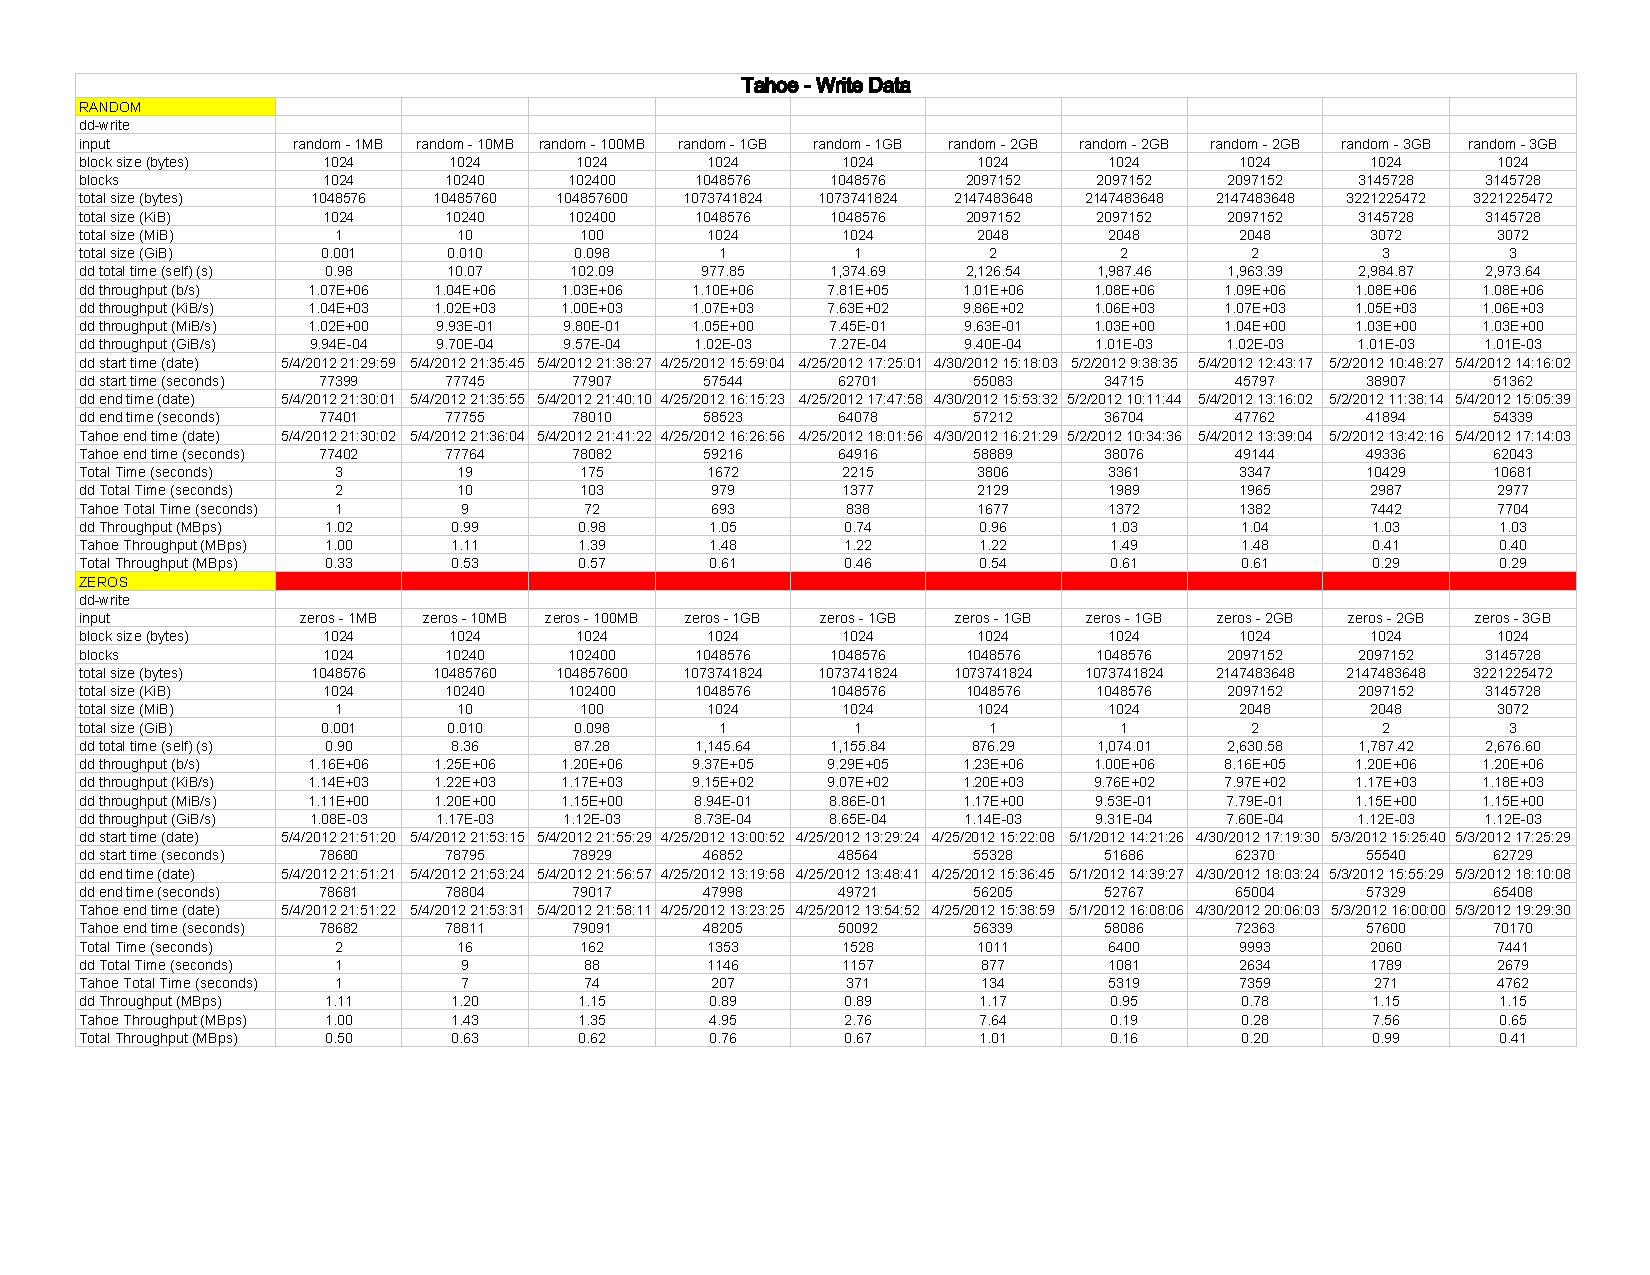
\includepdf[pages={1}, landscape]{include/TahoeWriteData.pdf}
\includepdf[pages={1}, landscape]{include/TahoeReadData.pdf}

\pagebreak
\section{Ceph Data}
\label{sec:CephData}

\pagebreak
\section{Lustre Data}
\label{sec:LustreData}

\pagebreak
\section{Tahoe Scripts}
\label{sec:TahoeScripts}

\lstinputlisting[
  float=htbp,
  caption={A simple script to call ssh and read password from file.},
  label=lst:sshpw
]{../code/tahoe/sshpw.sh}

\lstinputlisting[
  float=htbp,
  caption={A script to start Tahoe on the Tahoe Testbed
    (see Figure \ref{fig:TahoeTestbed})},
  label=lst:start-tahoe
]{../code/tahoe/start-tahoe-all.sh}

\lstinputlisting[
  float=htbp,
  caption={A script to stop Tahoe on the Tahoe Testbed
    (see Figure \ref{fig:TahoeTestbed})},
  label=lst:stop-tahoe
]{../code/tahoe/stop-tahoe-all.sh}

\lstinputlisting[
  float=htbp,
  caption={A script to start Tahoe on XPC1
    (see Figure \ref{fig:TahoeTestbed}},
  label=lst:start-tahoe-xpc1
]{../code/tahoe/tahoe-script/start-tahoe-xpc1.sh}

\lstinputlisting[
  float=htbp,
  caption={A script to start Tahoe on XPC2
    (see Figure \ref{fig:TahoeTestbed}},
  label=lst:start-tahoe-xpc2
]{../code/tahoe/tahoe-script/start-tahoe-xpc2.sh}

\lstinputlisting[
  float=htbp,
  caption={A script to start Tahoe on XPC3
    (see Figure \ref{fig:TahoeTestbed}},
  label=lst:start-tahoe-xpc3
]{../code/tahoe/tahoe-script/start-tahoe-xpc3.sh}

\lstinputlisting[
  float=htbp,
  caption={A script to stop Tahoe on XPC1
    (see Figure \ref{fig:TahoeTestbed}},
  label=lst:stop-tahoe-xpc1
]{../code/tahoe/tahoe-script/stop-tahoe-xpc1.sh}

\lstinputlisting[
  float=htbp,
  caption={A script to stop Tahoe on XPC2
    (see Figure \ref{fig:TahoeTestbed}},
  label=lst:stop-tahoe-xpc2
]{../code/tahoe/tahoe-script/stop-tahoe-xpc2.sh}

\lstinputlisting[
  float=htbp,
  caption={A script to stop Tahoe on XPC3
    (see Figure \ref{fig:TahoeTestbed}},
  label=lst:stop-tahoe-xpc3
]{../code/tahoe/tahoe-script/stop-tahoe-xpc3.sh}

\end{document}
